%%%%%%%%%%%%%%%%%%%%%%%%%%%%%%%%%%%%%%%%%%%%%%%%%%%%%%%%%%%%%%%%%%%%
%% I, the copyright holder of this work, release this work into the
%% public domain. This applies worldwide. In some countries this may
%% not be legally possible; if so: I grant anyone the right to use
%% this work for any purpose, without any conditions, unless such
%% conditions are required by law.
%%%%%%%%%%%%%%%%%%%%%%%%%%%%%%%%%%%%%%%%%%%%%%%%%%%%%%%%%%%%%%%%%%%%

\documentclass[
  digital, %% The `digital` option enables the default options for the
           %% digital version of a document. Replace with `printed`
           %% to enable the default options for the printed version
           %% of a document.
%%  color,   %% Uncomment these lines (by removing the %% at the
%%           %% beginning) to use color in the printed version of your
%%           %% document
  oneside, %% The `oneside` option enables one-sided typesetting,
           %% which is preferred if you are only going to submit a
           %% digital version of your thesis. Replace with `twoside`
           %% for double-sided typesetting if you are planning to
           %% also print your thesis. For double-sided typesetting,
           %% use at least 120 g/m² paper to prevent show-through.
  lof,     %% The `lof` option prints the List of Figures. Replace
           %% with `nolof` to hide the List of Figures.
  lot,     %% The `lot` option prints the List of Tables. Replace
           %% with `nolot` to hide the List of Tables.
]{fithesis4}
%% The following section sets up the locales used in the thesis.
\usepackage[resetfonts]{cmap} %% We need to load the T2A font encoding
% \usepackage[T1,T2A]{fontenc}  %% to use the Cyrillic fonts with Russian texts.
\usepackage[
  main=english, %% By using `czech` or `slovak` as the main locale
                %% instead of `english`, you can typeset the thesis
                %% in either Czech or Slovak, respectively.
  english, czech %% The additional keys allow
]{babel}        %% foreign texts to be typeset as follows:
% \usepackage[utf8x]{inputenc}
\usepackage[utf8]{inputenc}

\inputencoding{utf8}
\DeclareUnicodeCharacter{0301}{\'{e}}
% \usepackage[cp858]{inputenx}
% \DeclareUnicodeCharacter{0160}{\v{S}}
% \DeclareUnicodeCharacter{04F1}{\"\cyru}
% \DeclareUnicodeCharacter{04F2}{\H\CYRU}
% \DeclareUnicodeCharacter{04F3}{\H\cyru}
% \usepackage{newunicodechar}
% \newunicodechar{�}{x}
% Šumperk
\usepackage{textcomp}

%% For non-Latin scripts, it may be necessary to load additional
%% fonts:
\usepackage{paratype}
% \def\textrussian#1{{\usefont{T2A}{PTSerif-TLF}{m}{rm}#1}}
%%
%% The following section sets up the metadata of the thesis.
\thesissetup{
    date        = \the\year/\the\month/\the\day,
    university  = mu,
    faculty     = fi,
    type        = mgr,
    department  = Department of Machine Learning and Data Processing,
    author      = {Ing. Štěpán Skovajsa},
    gender      = m,
    advisor     = {RNDr. Petr Novotný, Ph.D.},
    title       = {Modelling of Infection Risk via Probabilistic Programming},
    keywords    = {Bayes theorem, Bayesian inference, statistics, Distribution function, Probabilistic programming, Probabilistic model, PyMC3, Monte-Carlo simulation, Hamiltonian Monte-Carlo, Covid-19, Epidemiology, Epidemiological risk, Infection, Disease, SIR model, Reproduction number},
    abstract    = {%
      In the epidemiology, there is no holy grail for modelling the risk of infection. Usually, the epidemiologists publish reports with daily incidence and reproduction numbers as a product of some epidemiologic model. Unfortunatelly, this indicator is less interpretable by common people. Moreover, these estimates of the reproduction numbers are, in most cases, approximated for wider geographical segments, usually whole states, ignoring spatial differences between regions. The primary cause is the ordinary models can't work with insufficient or very noisy data (i.e. zero-inflated daily incidence).

      This thesis provides robust probabilistic mathematical model and Monte Carlo solution for determining the systematic risk of encountering infectious individual given the number of contacts in individual geographic areas. Also the minimal required theory for understanding the approach is presented.

      Although the probabilistic model is tuned for modelling the risk of being infected by Covid-19 in specific districts of the Czechia, it might be, with little adjustment, used for modelling other epidemies as well.
    },
    thanks      = {%
      I would like to thank to my supervisor, RNDr. Petr Novotný,~Ph.D.,~especially for introducing me into probabilistic modeling and for the challenge I was able to take by choosing this thesis proposal. Also for his guidance, support and valuable advices, he provided for entire process. I would also like to thank to every author of each title mentioned in bibliography for their work, so I was able to built this thesis. And also, I won't forget to thank to my family and girlfriend for their endless support.
    },
    bib         = references.bib,
    %% Remove the following line to use the JVS 2018 faculty logo.
    facultyLogo = fithesis-fi,
}
\usepackage{makeidx}      %% The `makeidx` package contains
\makeindex                %% helper commands for index typesetting.
% \usepackage[acronym]{glossaries}          %% The `glossaries` package
% \renewcommand*\glspostdescription{\hfill} %% contains helper commands
% \loadglsentries{example-terms-abbrs.tex}  %% for typesetting glossaries
% \makenoidxglossaries                      %% and lists of abbreviations.
%% These additional packages are used within the document:
\usepackage{paralist} %% Compact list environments
\usepackage{amsmath}  %% Mathematics
\DeclareMathOperator*{\argmax}{arg\,max}
\DeclareMathOperator*{\argmin}{arg\,min}
\usepackage{amsthm}
\usepackage{amsfonts}
\usepackage{amssymb}
\usepackage{url}      %% Hyperlinks
\makeatletter
\g@addto@macro{\UrlBreaks}{\UrlOrds}
\makeatother
\usepackage{markdown} %% Lightweight markup
\usepackage{listings} %% Source code highlighting
\lstset{
  basicstyle      = \ttfamily,
  identifierstyle = \color{black},
  keywordstyle    = \color{blue},
  keywordstyle    = {[2]\color{cyan}},
  keywordstyle    = {[3]\color{olive}},
  stringstyle     = \color{teal},
  commentstyle    = \itshape\color{magenta},
  breaklines      = true,
}
\renewcommand{\lstlistingname}{Snippet}
\usepackage{floatrow} %% Putting captions above tables
\floatsetup[table]{capposition=top}
\usepackage[babel]{csquotes} %% Context-sensitive quotation marks
\begin{document}
%% Uncomment the following lines (by removing the %% at the beginning)
%% and to print out List of Abbreviations and/or Glossary in your
%% document. Titles for these tables can be changed by replacing the
%% titles `Abbreviations` and `Glossary`, respectively.
%% \clearpage
%% \printnoidxglossary[title={Abbreviations}, type=\acronymtype]
%% \printnoidxglossary[title={Glossary}]

%% The \chapter* command can be used to produce unnumbered chapters:
\chapter*{Introduction}
%% Unlike \chapter, \chapter* does not update the headings and does not
%% enter the chapter to the table of contents. I we want correct
%% headings and a table of contents entry, we must add them manually:
\markright{\textsc{Introduction}}
\addcontentsline{toc}{chapter}{Introduction}

Epidemiology subsumes several science disciplines like biology, 
math, social sciences, etc. 
It is caused by the nature of an epidemic disease - it is 
invisible for our eyes, but might have significant impact on 
our health and the society as a whole.
From the bottom of matter, it may start with investigating a 
disease from the microbiological perspective in a laboratory, 
through disease tracking of infected people and sudden mathematical
modelling, ending  with government interventions like social distancing, 
healthcare crisis management, vaccination strategy, financial and other 
support for most affected segments or areas.

The above-mentioned mathematical modelling may be used in 
various perspectives for the epidemiology. It may be used to
better understand how a disease is spread, what is the risk 
of being infectious or succumb to a disease. In that medical 
perspective, the mathematical modelling provides foundation to 
prevent the spread of a disease, or at least, to minimalize health damage.
On the other hand, the mathematical modelling can also be used to model
socio-economical impact due to lockdowns, quarantine 
and for modelling business decisions during pandemic.

In both perspectives, it uses medical and statistical data about a 
disease, demographic and socio-economic data about population, 
their transitivity between regions, etc. 
Also methods for finding solutions are quite similar. 
The main difference between those perspectives lies in the model, 
which is the mathematical formulation of a problem to be solved. 
Unfortunatelly, it is quite difficult to take into count all 
possible cases and situations, especially when there are not 
good enough data, so it is unrealistic to model disease exactly. 
Instead of this, we do approximations of the real world 
with best data available and given precision.

The basic reproduction number $\mathcal{R}_0$ and the effective 
reproduction number $\mathcal{R}_e$ are often parts of reports 
published by epidemiologists and other related experts.
For common people (i.e. non-epidemiologists) those indicators 
may be insufficient or incomprehensible in the basic sense.
Moreover, those indicators are usually reported for whole contries, 
not for lower administrative units such as cities, districts or regions. 
For these reasons this thesis present more human friendly 
probabilistic approach to model systematic epidemic risk of
infectious contact.


\chapter{The risk as a probability}
\label{chap:risk-as-probability}

The risk itself can be, in very general taxonomy, seen from
\textit{idiosyncratic} and \textit{systematic} perspective.
\textit{Systematic risk} is the more general one, it affects everyone, 
or at least, everyone in the very large sample considerable as a population
(e.g., citizens of a city, disease-susceptible seniors in country).
In contrary, the \textit{idiosyncratic risk} is the specific (individual) type of risk,
which is more focused on small sample of individuals.
Good example of idiosyncratic risk are superspreaders, the infected
individuals with usually low frequency of occurrence, but with ability to
infect excessive amount of people \cite[Chapter~4]{brauer2008}.
This makes idiosyncratic risk more difficult to grasp, therefore, 
we will focus on the systematic risk only.

In the quantitative risk assessment way of thinking, the risk can be
perceived as a probability \cite[Chapter~14]{bahr2014}.
In our case, the risk we model will be a 
probability of infectious contact. This mean, we are 
looking for probability of meeting at least one
infected individual given the number of random contacts:

\begin{equation}\label{eq:risk-first}
  \text{risk} = P(\text{infectious contact} | \text{number of contacts})
\end{equation}

Let $N$ denote the size of population and $I$ the number of infected
individuals among that population, thus $I \leq N$.
Assuming the infectious $I$ are uniformly distributed
across population, $p = \frac{I}{N}$ is the probability of
selecting infected individual.
This corresponds to the \textit{Bernoulli 
distribution} \cite{bernoulli-dist}:

\begin{equation}
  X \sim \text{Bernoulli} \left( p \right)
\end{equation}

where $X$ corresponds to the dichotomous random variable
($X = 1 \Rightarrow \text{infectious}$, $X = 0 \Rightarrow \text{non-infectious}$).

Now lets bring the \textit{number of contacts} from 
\eqref{eq:risk-first} into the computation.
This quantity can be imagined as a size of the sample of people
the investigated individual (the one for whom we compute the risk)
have met previously.
If we denote the size of this sample $n$, we are basically interested
in the number of infected individuals $i$ in that sample such 
that $i \leq n$. We can rewrite \eqref{eq:risk-first} as:

\begin{equation}\label{eq:risk-second}
  P(i \geq 1 | n)
\end{equation}

As we assume $i$ to be discrete random variable,
the discrete probabilistic distributions should be considered.
Namingly \textit{binomial}, \textit{negative binomial} and 
\textit{hypergeometric} distributions.

Both the binomial and negative binomial distributions
are built on top of independent Bernoulli trials.
This assumes the probability $p$ of selecting each particular
individual is same.
This is theoretically not true for our case, because we
are basically taking samples without replacement.
This means the probability of choosing each individual
changes during the sampling process, i.e., sampled 
individual is no longer part of the remaining
population to sample from. This is valid for
\textit{hypergeometric distribution} \cite{hypergeometric-dist}.
Therefore, the \textit{probability mass function} for $i$ given the
$N$, $I$ and $n$ will be:

\begin{equation}
  p(i|n) = \frac{ \binom{I}{i} \binom{N - I}{n - i} }{ \binom{N}{n} }
\end{equation}

where $\binom{a}{b}$ is a binomial coefficient.
We assume the validity of the p.m.f. for the condition
$max\left( 0, I - N + n \right) \leq i \leq min\left( I, n \right)$.
However, p.m.f. is a probability that exactly $i$
infected individuals occupy the sample.
For sure, we can use cumulative distribution functions
to expressing probability of $i$ or less, but, 
in our case, we want to invert this probability,
i.e., expressing there is at least $i$ infectious in the sample.
Normally, we would do something like $1 - P(X \leq x)$,
but we can image the probability of one and more
infected individuals as an inverted probability that
no one is infected, therefore, the risk 
probability may be assumed as:

\begin{equation}\label{eq:risk-theoretic}
  P(i \geq 1|n) = 1 - p(i=0|n) = 1 - \frac{
    \binom{N - I}{n}
  }{
    \binom{N}{n}
  }
\end{equation}

As the $N$ and $n$ are known values, and $i$ the quantity, for 
which, the probability we want to know, the 
remaining question is how to approach value of $I$.

Fortunatelly, this thesis provides the probabilistic solution,
but before we dive in, we have to introduce
epidemiological fundaments first, because every data science
project requires particular \textit{domain knowledge} to
understand problem deeply, and this is not an exception.


\chapter{Epidemiological prerequisites}
\label{chap:epidemiological-prerequisites}

This chapter provides basic insight into the mathematical
epidemiology, 
i.e., history of mathematical modelling to highlight gradual 
development of mathematical methods, basic terminology 
used both in epidemiology and this thesis, and the most 
basic mathematical models.
Following basic epidemiologic 
overview will help to understand the whole concept how 
the solution was build.

During the gradual development of history,
the people registered several deadly diseases of unknown origin.
Then survivors tended to investigate causes of those 
fatalities to avoid future outbreaks, or at least, mitigate its effects.
In that sense, the science about disease spread 
prevention has started to arising.
\textit{U.S. Department of Health and Human Services Centers 
for Disease Control and Prevention} (\textit{CDC}) provides the 
following definition for \textit{epidemiology} \cite{cdc2006}:

\begin{displayquote}
  ``Epidemiology is the study of the distribution and
  determinants of health-related states or events in specified
  populations, and the application of this study to the control
  of health problems.''
\end{displayquote}

Nowadays, the mathematical modelling is necessary 
step when disease outbreak occurs, starting with computation 
of $\mathcal{R}_0$ (more on this later) to reveal severity 
of the disease.
Later then, it helps with decision 
making during the pandemic state, keeping population safe 
according to health, economy and social amenities.


\section{History of mathematical modelling in epidemiology}

The first study of this type considered was the book 1663 by 
John Graunt addressing methods of public health statistics.
In 1766, Daniel Bernoulli was analyzing smallpox in his work 
considered to be the first epidemiological model.
Then, the biological aspects of viruses and diseases was 
studied primarily by leading scientists of the time.
Those significant names include Louis Pasteur and Robert Koch.
The mathematical modelling contributions were done later in
the early twentieth century \cite[Chapter~1.4]{martcheva2015}.
William Hamer was the first who used the law of 
mass action for modelling recurrence of measles. 
Sir Ronald Ross is considered to be the founder of 
modern mathematical epidemiology due to his contribution
to mathematical modelling of malaria
transmission. He derived a threshold quantity, which is 
nowadays known as a \textit{basic reproduction number}
denoted by $\mathcal{R}_0$.
Unfortunately, at his times, the mathematical modelling 
of diseases was not very accepted by the professional community.
The change of mind in this field was bring by the invention 
of mathematical foundations of compartment models
(SIR model to be more specific) in 1927 by W. O. Kermack and 
A. G. McKendrick \cite{kermack1927}.



\section{Epidemiological glossary}

The picture \ref{fig:epidemiologists-bathtub} explains the most basic
terms such as \textit{incidence}, \textit{prevalence}, \textit{mortality}
and \textit{recovery} in the bathtub analogy:

\begin{figure}[h]
  \begin{center}
    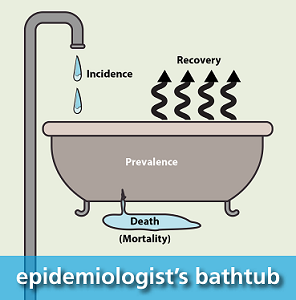
\includegraphics[width=8cm]{static/images/epidemiologists-bathtub.png}
  \end{center}
  \caption{The bathtub analogy \cite{steward2020}}
  \label{fig:epidemiologists-bathtub}
\end{figure}

Let the bath represent a
set of infected people (those who are infectious) in certain time.
The size of this set is so-called \textit{prevalence} (sometimes also referred 
as \textit{active cases} number) for that time.
The prevalence can be \textit{increased} or \textit{decreased} when time is shifted upwards.
The increase is referred as the \textit{incidence} (will be mostly denoted $c$ here).
The decrease of prevalence may be done in two ways:
the infected individual dies - increase in \textit{mortality}, or, the
infected individual get restored from the disease - \textit{recovery} increase.
If we do not distinguish the way of decrease, we say the
individual was \textit{removed}.

Basically, from the perspective of specific case, the disease is
transmitted between \textit{infector} $A$ and \textit{infectee} $B$.
The \textit{infector} (also known as \textit{primary case}) is the one who carry the disease and
\textit{infectee} (also known as \textit{secondary case}) is the 
susceptible person, which is being infected.
We assume also \textit{infection age} (denoted $a$ here),
which is the time for how long the specific individual is infected.
Basically, if the infector $A$ infects infectee $B$, it is done at infector's
infection age $a_A > 0$, and when the transmission of infection suceed,
the infectee starts its own infection age $a_B = 0$.
This abstraction allows to specify several important time intervals.

\begin{figure}[H]
  \begin{center}
    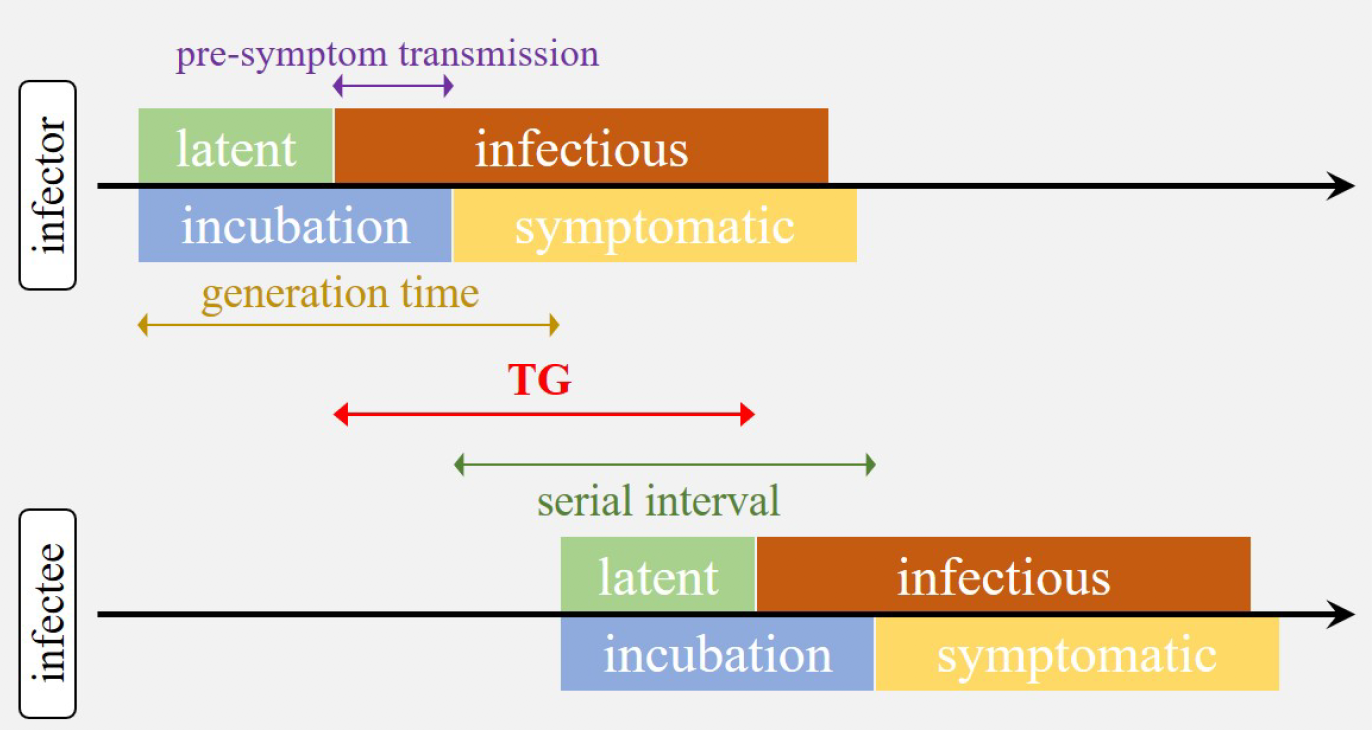
\includegraphics[width=11cm]{static/images/zhao2020_terms.png}
  \end{center}
  \caption{The demonstrative timeline of a transmission chain for a pair of infector and infectee \cite{zhao2020}}
  \label{fig:zhao-transmissive-chain-example}
\end{figure}

Most important time intervals are 
\textit{incubation period} $h$, \textit{serial interval} $s$ and \textit{generation time} $g$.
\textit{Incubation period} is the time between exposure up to time of onset 
symptoms. In this period, infected is usually not aware about his infection.
It is revealed later when \textit{symptomatic period} began.
\textit{Generation time} is the exact time period between time
the infector was infected and time the infectee was infected by the infector.
The \textit{serial interval} has similar nature. It is 
the time period between the onset symptoms of the infector 
and onset symptoms noticed on the associated infectee.

% TG, also in the picture \ref{fig:zhao-transmissive-chain-example}, abbreviates 
% \textit{trasmission generation}, which is the time 
% period between the infectiousness of the infector 
% and the infectousness of the infectious, meaning 
% how many susceptibles can be infected from the 
% primary case until the associated secondary case can 
% be transmissibe as well.

When the infector infects the infectee before the infector's
symptoms appear, we call it \textit{presymptomatic transmission}, i.e.,
infectee was infected in infector's \textit{incubation period}
(as shown in the figure \ref{fig:nishiura-transmission}).

When $s < 0$ the infectee's symptoms occurred earier than infector's.
On the other hand, $g > 0$ is always
valid, because the infector is always infected earlier than infectee.

\begin{figure}[h]
  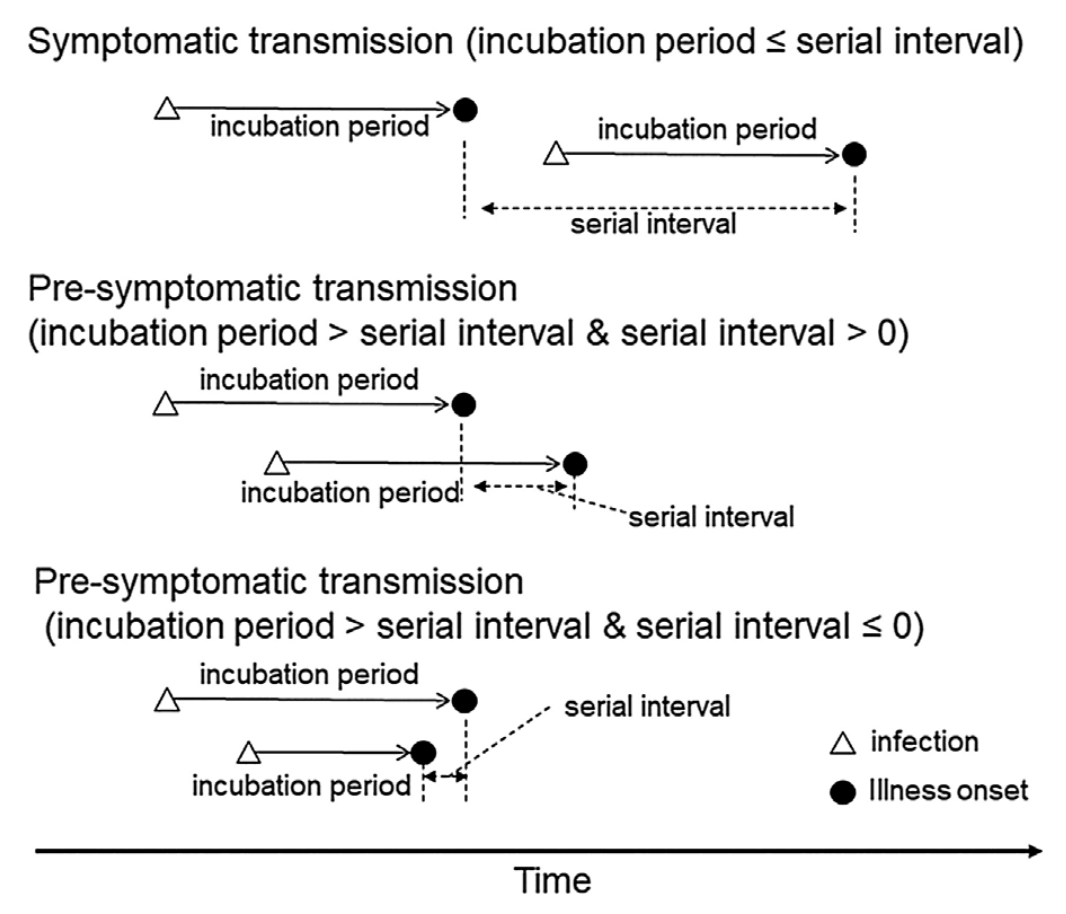
\includegraphics[width=10cm]{static/images/nishiura2020_terms.png}
  \caption{The relationship between the incubation period and serial interval. \cite{nishiura2020}}
  \label{fig:nishiura-transmission}
\end{figure}

% In many cases, the serial interval for modeling $\mathcal{R}_t$ 
% is used because of its easier determination. 
% The main pitfall lies in the possibility of negative serial 
% interval, that is when infectee's symptoms are revealed 
% earlier than infector's. 
% On the other hand, generation time has to be higher than 
% zero in its nature, but it is unknown in many cases. 

% For example \cite{knight2020} uses deconvolution of incubation 
% period and serial interval to obtain generation time.



\section{Kermack–McKendrick model}

This is one of the first well-known model (generally 
known as \textit{SIR model}), proposed in 1927 by 
William Ogilvy Kermack and Anderson Gray McKendrick, and is 
usually used as an introductionary model to epidemic 
modeling \cite{martcheva2015} due to its simplicity, and
often serves as a foundation for more complex 
models (\cite{clancy2008} for example).

The SIR model divides entire population into three disjunct 
sets, called \textit{classes} or \textit{compatments} (hence the general 
name \textit{compartment models} \cite{bacaer2011}):

\begin{itemize}
  \item \textit{Susceptibles (size denoted $S$)} - set containing non-infected individuals, but with possibility to become infected.
  \item \textit{Infectious (size denoted $I$)} - individuals who are infected and also able to infect susceptible individuals.
  \item \textit{Recovery / Removed (size denoted $R$)} - those who was restored from illnes (and gained immunity) or those who died. In both cases, they are removed from susceptibles and infectious sets, and therefore, they do not play any further role.
\end{itemize}

To define the SIR model, let us explain the \textit{force of infection} first.
The force of infection, noted $\lambda$, is similar to 
potential energy in physics, in this case, it expresses 
potential spreading force of the infectious compartment:

\begin{equation}
	\lambda = \tau \rho I
\end{equation}

Where $\rho$ is the average contact rate of person within whole 
population, no matter if they are susceptible, infectious 
or removed.
Let $N$ be the size of population,
then $\rho N$ is the \textit{average number of contacts}.
Assuming the susceptibles are independently and identically 
distributed, the probability of selecting any susceptible 
in the population is equal to $\frac{S}{N}$.
Therefore $\rho N\frac{S}{N}$ is the number of contacts 
each infected individual makes with susceptibles 
(simplifies to $\rho S$).
$\tau$ is the probability of becoming infectious for 
susceptible, which met an infected individual:

\begin{equation}
	\tau = p \left( B~\textrm{is infected from}~A~|~B~\textrm{has contact with}~A \right)
\end{equation}

If the previous equations are combined together, 
$\tau \rho S$ can be assumed as the number of 
susceptibles who became infectious after they have 
met one infected individual per unit of time.
Now the incidence may be formulated as:

\begin{equation}
	c = \tau \rho I \frac{S}{N} = \lambda \frac{S}{N}
\end{equation}

For practical usages denote $\tau \rho$ as $\beta$ 
and substitute it into previous equation to get:

\begin{equation}
	c = \beta I \frac{S}{N}
\end{equation}

The compartment models are usually specified as a set of
differential equations. Lets start with the susceptibles
compartment $S$. In the basic SIR model, the $S$
can be decresed only (as it assumes the everyone can be 
infected only once).
This decrease is equal to the incidence, hence:

\begin{equation}\label{eq:sir-model-incidence}
	\frac{\partial{S}}{\partial{t}} = -c = -\beta I \frac{S}{N}
\end{equation}

The decrease of susceptibles $\beta I \frac{S}{N}$ is basically 
count of the newly infected individuals, which have 
to be added to $I$. 
Then, some of the infected individuals restore from 
the infection, or decease. 
This proportion is equal to $\gamma I$, where $\gamma$ 
is called \textit{recovery rate}. Both increase and decrease in 
the $I$ compartment is caught in equation:

\begin{equation}\label{eq:sir-model-partial-I}
	\frac{\partial{I}}{\partial{t}} = \beta I \frac{S}{N} - \gamma I
\end{equation}

Finally, the decreased proportion $\gamma I$ from the 
$I$ compartment increases removed compartment $R$:

\begin{equation}
	\frac{\partial{R}}{\partial{t}} = \gamma I
\end{equation}

This model has several assumptions:

\begin{enumerate}
  \item Population is constant over time \\
    \begin{equation}
      N = S(t) + I(t) + R(t) = const.
    \end{equation} \\
    Therefore: \\
    \begin{equation}
      \frac{\partial{S}}{\partial{t}} + \frac{\partial{I}}{\partial{t}} + \frac{\partial{R}}{\partial{t}} = 0
    \end{equation}
  \item When susceptible gets infected, it also becomes infectious
  \item Each susceptible has equal probability to become infectious
  \item Everyone can be infected only once in his lifetime
  \item There is no latent period, once the transmission of infection is done, the infectee is infectious instantaneously (in continuous model)
  \item Each infected individual is equally infective \cite{volz2018}
\end{enumerate}

As a summary comparable statistics, the $\beta$ and $\gamma$
may be used, but epidemiologists rather compare 
reproduction numbers, which are much more general.


\section{Reproduction number}

The \textit{basic reproduction number} $\mathcal{R}_0$ is number 
of secondary cases caused by the one infectious individual 
in the completely susceptible population and can be expressed
as the following proportion \cite{jones2007}:

\begin{equation}
	\mathcal{R}_0 \propto \left(\frac{infection}{contact}\right)\cdot\left(\frac{contact}{time}\right)\cdot\left(\frac{time}{infection}\right)  
\end{equation}

In terms of SIR model defined above, and the fact $\gamma^{-1}$ is 
the average time of infection \cite{ma2019}, the following formula can be derived:

\begin{equation}
	\mathcal{R}_0 = \tau \rho d = \frac{\beta}{\gamma}
\end{equation}

Note the dimensionlessness of the $\mathcal{R}_0$.

The \textit{effective reproduction number} $\mathcal{R}_e$ 
($\mathcal{R}_{\text{t}}$, $\mathcal{R}_{\text{eff}}$ in 
some literature) is the average number of secondary cases 
caused by one infected individual within the 
conditions of time $t$ in the ongoing epidemic \cite{chowell2016}:

\begin{equation}
  \label{eq:sir-effective-reproduction-number}
	\mathcal{R}_e(t) = \mathcal{R}_0 \frac{S(t)}{N} = \frac{\beta}{\gamma} \frac{S(t)}{N}
\end{equation}

The basic reproduction number $\mathcal{R}_0$ is usually used
in the early epidemic phase to determine transmission potential.
When infection is
spreading through a population, it is often more convenient
to work with the effective reproduction number $\mathcal{R}_e(t)$.


\section{Exponential model}

The exponential model (also known as \textit{Malthusian} model, named after the 
Reverend Thomas Malthus\footnote{\url{https://cs.wikipedia.org/wiki/Thomas_Robert_Malthus}})
is based on the assumption that a change in the population 
is proportional to its size \cite{martcheva2015}:

\begin{equation}\label{eq:malthusian-diff}
  \frac{\partial N}{\partial t} = b N - d N
\end{equation}

where $b$ is a birth rate and $d$ is a death rate, which 
can be extracted to the \textit{exponential growth rate} $r = b - d$.
The solution for differential equation \eqref{eq:malthusian-diff} is therefore:
\begin{equation}
  N(t) = N(0) e^{(b - d)t} = N(0) e^{rt}
\end{equation}

If $r > 0$ the population is growing,
if $r = 0$, then population remains constant, and finally, 
when $r < 0$ the population leads to extinction.

We can utilize exponential model,
for example, in the early epidemic phase,
where $\forall u \in (0, t) : S(u) \approx N$, so we can assume $\frac{S}{N} = 1$,
and, after replacing population $N$ for infectious $I$, we get:

\begin{equation}
  \frac{\partial I}{\partial t} = b I - d I
\end{equation}

If we also replace $b$ for $\beta$ and $d$ for $\gamma$, we
obtain exacty the equation \eqref{eq:sir-model-partial-I} for $\frac{S}{N} = 1$ in the SIR model.
Therefore, in the early phase of epidemic, it holds:

\begin{equation}
  I(t) = I(0) e^{rt}
\end{equation}

where $r = \beta - \gamma$ is exponential growth rate for the early epidemic
if the SIR model is used \cite{ma2019}.

% and infectious time is assumed to be exponentially distributed


\section{Wallinga \& Lipsitch model}
\label{sec:wl-model}

Wallinga and Lipsitch \cite{wallinga2007} developed a non-parametric
model (shortened as \textit{WL model} here), which is able to infer
the basic reproduction number from the \textit{exponential growth rate} $r$.

This model is based on the exponential growth model described earlier and
Euler-Lotka equation\footnote{\url{https://en.wikipedia.org/wiki/Euler\%E2\%80\%93Lotka_equation}},
which was originally used to model population dynamics.
Let the $b(t)$ be the number of female births at the time $t$, $a$ is 
age of the mother (assuming population has sufficient 
number of males to ensure reproduction, therefore we do not 
count them in), and $n(a)$ is the rate of production of female offsprings 
by one mother at her age $a$. Then we have this equation (which is 
special type of renewal equation \cite{feller1941}):

\begin{equation}\label{eq:wl-model-renewal}
  b(t) = \int_{0}^{\infty} b(t - a) n(a) da
\end{equation}

If we sum up the $n(a)$ in the equation, we obtain \textit{reproductive number} 
$\mathcal{R}$ expressing the total number of female offsprings from one mother:

\begin{equation}\label{eq:wl-model-R}
  \mathcal{R} = \int_0^{\infty} n(a) da
\end{equation}

As the $b(t)$ is assumed to follow exponential growth model, then 
the $b$ functions can be assumed $b(t) = Q e^{rt}$ and 
$b(t - a) = Q e^{r(t - a)} = Q e^{rt} e^{-ra}$, therefore the
previous equation may be rewritten to:

\begin{equation}
  Q e^{rt} = \int_{0}^{\infty} Q e^{rt} e^{-ra} n(a) da
\end{equation}

Note the $Q e^{rt}$ on both sides. At the side of integral, 
as this expression is independent of $a$, i.e., constant, we can 
divide both sides by this constant to obtain Euler-Lotka
equation (in the original equation $n(a) = l(a) m(a)$, but 
here is intentional simplification):

\begin{equation}\label{eq:wl-model-euler-lotka}
  1 = \int_{0}^{\infty} e^{-ra} n(a) da
\end{equation}

To incorporate $\mathcal{R}$ we can normalize the $n(a)$, in the
previous equation, by the equation \eqref{eq:wl-model-R} to get
normalized distribution $\omega(a)$ (note $\omega(a)$ becomes 
probability density function):

\begin{equation}
  \omega(a) = \frac{n(a)}{\int_0^{\infty} n(a) da} = \frac{n(a)}{\mathcal{R}}
\end{equation}

Now the previous may be employed in the equation \eqref{eq:wl-model-euler-lotka}:

\begin{equation}\label{eq:wl-model-euler-lotka-R}
  \frac{1}{\mathcal{R}} = \int_{0}^{\infty} e^{-ra} \frac{n(a)}{\mathcal{R}} da = \int_{0}^{\infty} e^{-ra} \omega(a) da
\end{equation}

Finally, we can obtain the formula for computation reproductive number
$\mathcal{R}$ from the exponential growth $r$ and reproduction profile $\omega$:

\begin{equation}\label{eq:wl-model-euler-lotka-R-final}
  \mathcal{R} = \frac{1}{\int_{0}^{\infty} e^{-ra} \omega(a) da}
\end{equation}

For the epidemiology, $\omega$ represents
a distribution of \textit{generation time} defined earlier.
The $\mathcal{R}$ is average number of new infectees from one infector
during its whole infection age (\cite{fraser2007} 
calls it \textit{instantaneous reproduction number}).
This approach works well in the early phases of epidemic,
when incidence grows exponentially
and proportion of susceptibles is not very drastically
changed $S(0) \approx N$ \cite{park2021}, then we can assume 
$\mathcal{R}_0 = \mathcal{R}$.


\section{Fraser model}
\label{sec:fraser-model}

The \cite{fraser2007} proposes model where the effective 
reproduction number $\mathcal{R}_e$ is computed from the 
daily incidence data and generation time only.

The approach of Fraser is very related to WL
model. In fact, it utilizes modified equation
\eqref{eq:wl-model-renewal}, where 
$n(a) = A(t, a)$ and $b(t) = c(t)$, therefore:

\begin{equation}
  c( t ) = \int^{\infty}_0 c ( t - a ) A ( t, a ) da
\end{equation}

The reason, infectiousness $A(t, a)$, in contrary to $n(a)$, 
depends on calendar time $t$ is, 
the epidemic may change its behavior in longer time period
(seasonality, government interventions, etc.).

For practical purposes, it is convenient to bound $a$ 
by specific $a_{max}$ which may correspond to the expected
maximal infection age, assuming nobody is infectious after 
$a_{max}$, therefore $A(t, a) = 0$ if $a > a_{max}$.
This leads to the next simplification.
For bounded $a \leq a_{max}$, where $a_{max}$ is 
sufficiently small, $A(t, a) = A(s, a)$ for 
$\forall s \in \left[ t - a_{max}, t \right]$.
Next, Fraser assumes that the seasonal infectivity is 
independent of infection age $a$ and vice versa, therefore
the transmissibility can be decomposed as:

\begin{equation}
A(t, a) = \phi_1(t) \phi_2(a)
\end{equation}

The average number of infected cases from the single infected 
individual can be obtained by summing over transmissibility:

\begin{equation}
  \mathcal{R}(t) = \int^{\infty}_0 A(t, a) da = \phi_1(t) \int^{\infty}_0 \phi_2(a) da
\end{equation}

The $\phi_1(t)$ and $\phi_2(a)$ might be reweighted as 
product $\phi_1(t) \phi_2(a)$, without loss of generality. 
Therefore $\int^{\infty}_0 \phi_2(a) da = 1$ may be assumed. 
This bring that $\mathcal{R} = \phi_1(t)$, while $\phi_2(a)$ 
is considered to be a distribution of infectivity $a$ ago, 
meaning idealised generation time distribution $\omega$. 
Therefore:

\begin{equation}
A(t, a) = \mathcal{R}(t) \omega(a)
\end{equation}

Putting it to the renewal equation the following is obtained:

\begin{equation}
  \begin{split}
    c(t) & = \int^{\infty}_0 \mathcal{R}(t) \omega(a) c(t - a) da \\
    & = \mathcal{R}(t) \int^{\infty}_0 \omega(a) c(t - a) da\\
    & = \mathcal{R}(t) \Lambda(t)    
  \end{split}
\end{equation}

where $\Lambda(t)$ denotes the integral.
To obtain $\mathcal{R}_e(t)$, we can just reorganize the previous equation:

\begin{equation}\label{eq:fraser-Re}
  \mathcal{R}_e(t) = \frac{c(t)}{\Lambda(t)} = \frac{c(t)}{\int^{\infty}_0 \omega(a) c(t - a) da}
\end{equation}

This approach was laterly adopted also by \cite{cori2013} where serial 
interval was used as an approximation of the generation time.
The approach of \cite{cori2013} was recommended also by \cite{gostic2020},
and \cite{hasan2020} used different method, however, they confirm the 
results of \cite{cori2013}.


\section{Summary}

In this chapter, the fundaments of epidemiology were established.
This will be useful in the next chapter, where we will investigate
the data, so we know now what to look for and how to use it in
the upcoming modelling.


% For practical usage, we will discretize the previous equation 
% and add $a_{max}$ boundary, because of assumption of maximal 
% infectious age to be $a_{max}$, and also because of discrete 
% observations:

% \begin{equation}
% c_t = \mathcal{R}_t \Lambda_t = \mathcal{R}_t \sum^{a_{max}}_{a=0} \omega(a) c(t - a)
% \end{equation}

% TODO: For the sake of simplicity, 


\chapter{The situation analysis}

The purpose of this chapter is to better understand the situation 
we want to model, describe the data as available evidence, and
formulate very basic approach, based on the data, which will be 
developed more thoroughly later.

The modelled infectious disease, \textit{Covid-19}, is an abbreviated 
term for \textit{coronavirus disease 2019}, the infectious disease 
caused by \textit{SARS-CoV-2} virus. 
In december 2019, it was the first time the virus was spotted, 
when several patients with pneumonia was hospitalized in the 
Wuhan, Hubei province in China. 
After the extraction of virus genome, it was discovered 
70\% similarity in genetic sequence with SARS-CoV, 
firstly appeared in China in 2002 (the fatality rate 
was 9.6\%) \cite{hui2019}.
This was the ignition for governments to start with mitigation 
actions.
Covid-19 had huge health and economical impact not only in 
Czechia, but in the whole world \cite{maital2020}, because of many victims
succumb to the diseases, many businesses bankrupt according
to lockdowns, children were prevented from attending
school, many people got depression or feel anxiety \cite{khan2020}, etc.


\section{Available data}
\label{sec:available-data}

In general, the model is strong as the input data provided.
As we want to approximate the risk among Czechia, the most 
relevant data assumed comes from the official authorities.
There is a Covid-19 reporting web 
portal\footnote{\url{https://onemocneni-aktualne.mzcr.cz/}} operated 
by the Ministry of Healthcare and developed by IHIS CR\footnote{Institute of Health Information and Statistics of the Czech Republic, \url{https://www.uzis.cz/}} 
and IBA LF MU\footnote{Institute of Biostatistics and Analyses at the Faculty of Medicine of the Masaryk University, \url{http://www.iba.muni.cz/}}, 
stating National Health Information System (NHIS), Regional Public 
Health Authorities (RPHAs) and Ministry of Healthcare as its 
data source. 
The source is based on the REST API\footnote{See snippet \ref{snip:data-incidence}}, 
is updated on daily basis and provides several 
dataframes for various geographical areas across time period $T$.
The lowest geographical granularity, for which the data are available, 
is per \textit{district}.
In the dataset, for each district $u$, the following considerable 
time series are available:
\textit{cumulative incidence} $Y_C^u = \{ y_{Ct}^u : t \in T \}$,
\textit{cumulative restored} $Y_R^u = \{ y_{R t}^u : t \in T \}$,
\textit{cumulative deceased} $Y_D^u = \{ y_{D t}^u : t \in T \}$.

Now, as we know the available data, we are able to think about 
proper approach.


\section{The data based approach}
\label{sec:data-based-approach}

As was mentioned in the \autoref{chap:risk-as-probability},
we are primarily looking for the \textit{prevalence} $I$ 
estimation $\hat{I}$. Moreover, we are now familiar with
the nature of the data we will work with, so it only remains
to interconnect the data with the theory from \autoref{chap:epidemiological-prerequisites},
in the most efficient way.

The most basic model, SIR, is very flexible, but highly dependent 
on its parametrization.
Note the WL model (\autoref{sec:wl-model}) and Fraser model
(\autoref{sec:fraser-model}) are conceived for
estimating reproduction number rather than prevalence
(in fact, the prevalence itself is not even present there).
As none of the previous theoretical models is directly applicable,
we have to modify them to be able to compute the prevalence
estimation.

Let recall, the $\omega(a)$ as a serial interval, represents
a probability density function of transmission across
the infection age $a$.
We will denote $\Omega$ the cumulative distribution function
of this serial interval:

\begin{equation}\label{eq:Omega-int}
  \Omega(a) = \int_{0}^a \omega(x) dx
\end{equation}

If we assume the one fictive infector is going to infect
just one infectee with $100\%$ certainty, at worst, at the
end of the infector's infection age $a = a_{max}$, then
$\Omega(a)$ represents a probability the infectee is infected
in the time less then $a$.
For our purposes it will be sufficient to invert this probability,
i.e., $1 - \Omega(a)$, and perceive it as a cumulative distribution
of infection age. Then we may assume the prevalence $I$ as the sum
of incidence and the probability the infection remains at its
age $a$:

\begin{equation}\label{eq:prevalence-int}
  I(t) = \int_0^{\infty} c(t - a) (1 - \Omega(a)) da
\end{equation}

When we solve the minimal $a$ such
that $1 - \Omega(a) = 0$, we obtain infection age $a$ for which
the infectious individual is not able
to infect anybody, i.e., the probability of transimission
is $0$ and infection ends.
Practically, we are trying to solve:

\begin{equation}
  a_{max} = \argmin_a \left| 1 - \Omega(a) \right|
\end{equation}

This can be easily achieved, when we assume some small $\delta$,
so we have to find minimal $a$ such that $1 - \Omega(a) = \delta$
to obtain $a_{max}$. This threshold will also help to limit
computational complexity.

This shifts the problem of finding prevalence $I$ to find
$c$ and $\Omega$. $\Omega$ from \eqref{eq:Omega-int} can 
be also discretized:

$\omega$, and therefore $\Omega$, can be obtained from the epidemiological
studies for the specific disease, Covid-19, in our case.
Now, lets explore the data more deeply to figure out how
to obtain $Y_c$ from the data.


\section{Data analysis}

We need only the incidence observations, therefore, we only
need to work with $Y_C$.
As the \autoref{sec:available-data} introduced, the observed time
series are in the cumulative form.
To obtain observed incidence $Y_c$,
we need just to decumulate the original observations:

\begin{equation}
  Y_{ct} = Y_{C(t + 1)} - Y_{Ct}
\end{equation}

The observed incidence $Y_c$ for the three largest 
cities\footnote{In fact, they are districts according to 
administrative/statistical subdivision, hence the inclusion in the districts datasets} in Czechia, 
namingly Prague, Brno and Ostrava, looks as 
follows\footnote{Generated by snippet 
\ref{snip:data-largest-cities-plot}}:

\begin{figure}[H]
  \begin{center}
    \includegraphics[width=\textwidth]{generated/images/data-largest-cities-plot.png}
  \end{center}
  \caption{Observed incidence in the largest cities of Czechia}
  \label{fig:largest-cities-incidence}
\end{figure}

From the previous plot, it is obvious the data are overloaded 
with noise. 
In the detail view, the weekly seasonal pattern can be observed. 
In the epidemiology, according to \cite{liu2021} and \cite{annunziato2020}, 
those oscillations may be associated to different capacities 
of testing and reporting delays due to the weekend effect. 
We will assume this also applies for the Czechia's case of 
Covid-19 reporting, as \cite{komenda2020} and corresponding web 
application authors describe the methods how the data are
being collected and processed.

We have took the 3 largest cities intentionally because they
are characterized with largest population, and therefore, the 
highest possible variation in the data, which is most convenient 
for the proper data analysis.


\subsection{Stationarity verification}

As those data correspond to the time series, the stationarity 
should be verified. 
This may be done by \textit{Augmented Dickey-Fuller} (\textit{ADF}) 
test \cite{dickey1979}. 
In the ADF test, the null hypothesis that a \textit{unit root} is 
present in a sample. 
If the unit root is present, the sample is non-stationary. 
Therefore, the alternative hypothesis is the stationarity of 
the given sample.

\input{generated/tables/data-adf-test-prague}

In general, \textit{p-value} is the probability that test statistic 
of unknown distribution has equal or less extreme values 
than unknown distribution of the sample, assuming \textit{null 
hypothesis} to be \textit{true}. In simple words, it is the strength 
of belief in the null hypothesis, in this particular case, the sample is 
non-stationary. 
As that value of p-value is higher than $5\% (0.05)$, we fail to reject 
the null hypothesis, arguing the observed incidence 
$Y_c^\text{(Prague)}$ was generated by a non-stationary 
process\footnote{See snippet \ref{snip:data-adf-test-prague}}. 
Of course, the ADF test should be done for $Y_c^\text{(Brno)}$ 
and $Y_c^\text{(Ostrava)}$ samples as well, 
see tables \ref{tab:data-adf-test-brno}, \ref{tab:data-adf-test-ostrava}\footnote{Created by snippet \ref{snip:data-adf-test-brno-ostrava}}.
The results found have the similar nature, i.e.,
the time series are non-stationary.

\subsection{Seasonality decomposition}
\label{sec:seasonality-decomposition}

In the previous subsection, we have found the incidence time 
series data for the three largest cities are non-stationary. 
This means the specific observations $y_{c}$ were not 
generated by the same process in every $t$, i.e., not with a stationary probability
distribution $p(y_c | t) = p(y_c)$, but with some \textit{dynamic process}. 
This brings us to go further and analyze the data more precisely. 
For this purposes, the seasonal decomposition may be applied 
(see snippet \ref{snip:data-seasonal-decomposition-figure}). 
This type of decomposition results in structural time series, 
where the input time series is decomposed into specific 
components.

In this case, the decomposition is done by computing 7 days
(according to the weekend effect) 
two-sided moving average as a trend component $T$, then the 
seasonal component $S$ and residual $\epsilon$ are derived\footnote{\url{https://www.statsmodels.org/dev/generated/statsmodels.tsa.seasonal.seasonal_decompose.html}}. 
How the components are inferred depends on the selected model 
of decomposition. There are two considerable types: 
\textit{additive} and \textit{multiplicative}.

The following figures shows decomposed daily incidence 
$\Delta C$ to structured time series components. 
First figure\footnote{Created by snippet \ref{snip:data-seasonal-decomposition-additive}} show the additive decomposition model, 
formally $Y_c = T + S + \epsilon$:

\begin{figure}[H]
  \begin{center}
    \includegraphics[width=\textwidth]{generated/images/data-seasonal-decomposition-additive.png}
  \end{center}
  \caption{Example of additive seasonal decomposition}
  \label{fig:seasonal-decomposition-additive}
\end{figure}

Similarly, the second figure\footnote{Created by snippet \ref{snip:data-seasonal-decomposition-multiplicative}}
shows the multiplicative decomposition, particularly $Y_c = T S \epsilon$:

\begin{figure}[H]
  \begin{center}
    \includegraphics[width=\textwidth]{generated/images/data-seasonal-decomposition-multiplicative.png}
  \end{center}
  \caption{Example of multiplicative seasonal decomposition}
  \label{fig:seasonal-decomposition-multiplicative}
\end{figure}

From the previous plots, we can see rather the multiplicative 
relationship, according to residual component $\epsilon$, 
which distinctly acts more stationary right in the 
multiplicative model. 
The multiplicative model imply the variance is proportional 
to the mean. This effect can be also visually checked  
in the raw data (figure \ref{fig:largest-cities-incidence}).

To conclude, the data analysis shown multiplicative 
relationship, rather than additive, between trend, seasonality and residual 
components in the incidence data. 
The input data are very noisy and non-stationary, which 
usually eliminates many simple and fast statistical methods. 


% They usually suffer from poor input data, so the data have 
% to be somehow preprocessed first, otherwise the poor 
% approximations are produced out of these methods.



\section{Population data}

For the risk estimation from the hypergeometric distribution
presented in \autoref{chap:risk-as-probability}, we need a population size 
$N$ in each investigated district.
Fortunatelly, this can be easily obtained from the official statistical data.
In the Czechia, there is 76 districts and the capital city Prague,
for which the population data can be obtained from the \textit{Czech
statistical office} (CZSO\footnote{\url{https://www.czso.cz/}}).
For more details, see snippet \ref{snip:data-node-instances}.


\section{Generation time}

% \texorpdfstring{$\omega$}{Lg}
Sometimes the literature uses \textit{generation time} and \textit{serial interval} interchangeably (\cite{wallinga2004} for example).
In fact, it is very difficult to find
proper \textit{generation time} because it is very unlikely to determine
exact moment the infectee was infected\footnote{For example, \cite{knight2020} 
uses deconvolution of serial interval and incubation period to obtain generation time.}.
Instead of that, the symptoms
are usually more available indicator, therefore, the
\textit{serial interval} is usually used as an approximation (\cite{griffin2010}, \cite{najafi2020}, \cite{cori2013}).

There is an evidence the Covid-19 has pre-symptomatic 
transmission \cite{ma2020}, which can even occur more frequently 
than symptomatic \cite{nishiura2020}.
According to \cite{du2020} (cited in \cite{knight2020}), the negative serial interval 
occurred in $12.6\%$ reported cases.
\cite{oran2020} mentions the approximation of $40\%$ to $45\%$ of 
infections to be asymptomatic.
From these findings, we can conclude the probability distribution of the
generation time of Covid-19 should have most of its mass distributed in the early
days of infection age.
The \cite{knight2020} compares using \textit{generation time} and 
\textit{serial intervals} (from various authors mentioned also here) 
to estimate $\mathcal{R}_e$ for Covid-19, where the difference
presented there is an acceptable bias for us.
This allows us to use \textit{serial interval} to approximate
\textit{generation time} while preserving the required precision.

To recall, the \textit{serial interval} (SI) $\omega$ is a time 
interval between onset symptoms on the infector and the 
infectee, and may be expressed as a univariate random variable. 
Although the SI definitely depends on the variant (mutation) of 
Covid-19, the several SI resources from various time periods are 
presented:

\begin{itemize}
  \item \textit{Simone} \cite{simone2020} assumes serial interval to be gamma 
  distributed, i.e. $\omega \sim Gamma(\alpha,\beta)$, where 
  $\alpha \sim N \left( 1.87, 0.26^2 \right)$ and 
  $\beta \sim N \left( 0.28, 0.04^2 \right)$ in Italia.

  \item \textit{Prete} \cite{prete2020} proposes $\omega \sim LogNormal(\mu, \sigma)$ 
  with $\mu = 1.09$ and $\sigma = 0.72$ according to the 
  studies in Brazil.

  \item \textit{Knight} \cite{knight2020} uses deconvolution 
  to obtain generation interval: $\omega \sim Gamma(\alpha, \beta), \alpha = 1.813, \beta = 2,199$.

  \item \textit{Du} \cite{du2020} proposes normally distributed serial 
  interval with $\mu = 3.96$ and $\sigma = 4.75$.

  \item \textit{Nishiura} \cite{nishiura2020} concludes 
  $\omega \sim LogNormal \left( \mu = 4.7, \sigma = 2.9 \right)$.
\end{itemize}

Those are presented the following figure\footnote{Created by snippet \ref{snip:data-serial-intervals-overview}}:

\begin{figure}[H]
  \begin{center}
    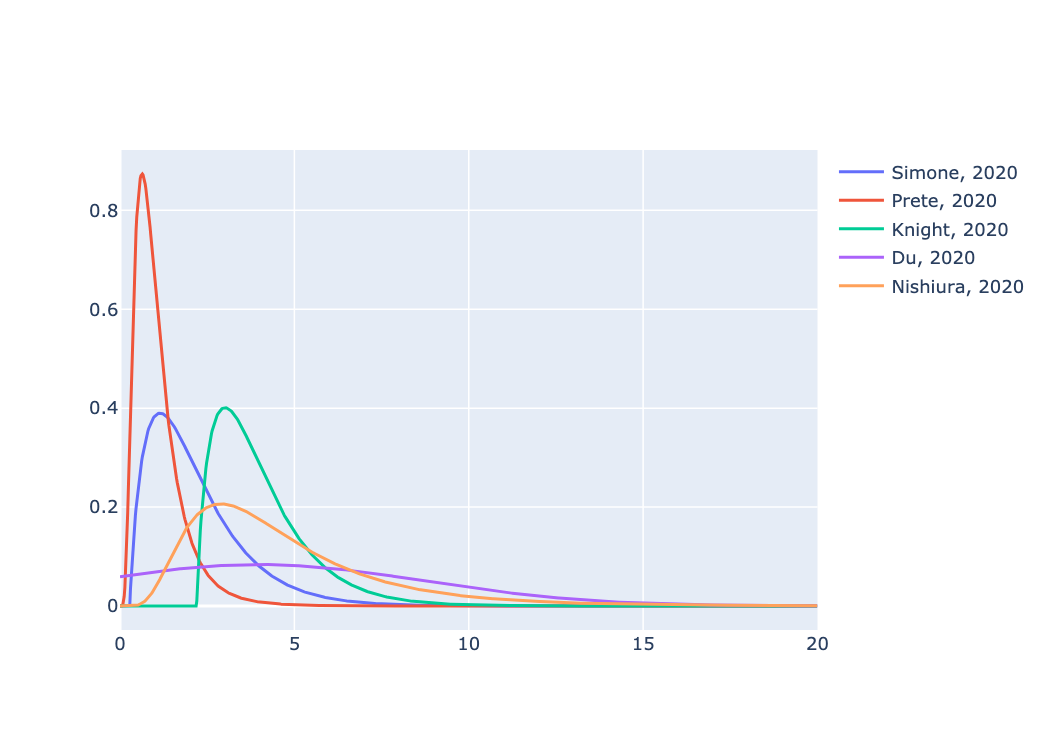
\includegraphics[width=\textwidth]{generated/images/serial-intervals-overview.png}
  \end{center}
  \caption{Referenced serial intervals}
  \label{fig:serial-intervals-overview}
\end{figure}

The previous serial intervals vary due to spatial and 
temporal differences in population composition and the
strain of the virus.
From the local research made by \cite{majek2020}, 
it is estimated the SI of Covid-19 for Czech republic is 4-5 days, which is 
stated to be consistent with \cite{nishiura2020}. 
In the time of writing this thesis, more precise work on the 
SI of predominant delta mutation could not be found. 
Therefore we will stick with \cite{majek2020} and 
\cite{nishiura2020} and assume 
$\omega \sim LogNormal \left( \mu = 4.7, \sigma = 2.9 \right)$ 
as the source of truth.

As we assumed $\omega$, we can easily compute $\Omega$ and 
make an assumption about $a_{max}$.
Let's plot the $1 - \Omega$:

\begin{figure}[H]
  \begin{center}
    \includegraphics[width=\textwidth]{generated/images/data-1-Omega.png}
  \end{center}
  \caption{$1 - \Omega$}
  \label{fig:data-1-Omega}
\end{figure}

Given the previous figure, we can safely assume 
$a_{max} = 10$ as sufficient.

% According to the chart above, we can put upper limit of the 
% infection age $a_{max}$ to $15$ days.

\section{Summary}

In this chapter, the situation was analyzed.
This means, we investigated the available
epidemic data, population data and available
serial interval to use as a generation time $\omega$.
We also derived the formula for prevalence calculation,
which depends on incidence $c$ and $\omega$.

For now, the only problem is the incidence $c$,
for whom the observed values $Y_c$ are available.
There is a huge noisiness in the data, which can be overcomed by using 
smoothing techniques.

\cite{elmousalami2020} compares deterministic
methods as the moving average, weighted 
moving average, single exponential smoothing for 
forecasting Covid-19, while these methods may be used 
for smoothing too. \cite{annunziato2020} draws attention to use smoothing 
methods carefuly as some oscillations might still remain in 
the input data from the improper data collection.

Therefore, it is very important to devote sufficient
amount of time to choose proper smoothing technique.
The next chapter is dedicated to the inference of
incidence estimation $\hat{c}$ from the observed 
incidence $Y_c$, i.e., denoise/smoothen $Y_c$ to $\hat{c}$, called
\textit{the incidence model}.


\chapter{The incidence model}

In the most basic taxonomy of mathematical models, they can be 
split into two main categories: \textit{deterministic} and 
\textit{probabilistic}, also known as \textit{stochastic}. 
Big advantage of deterministic models is their 
straightforwardness and lower computational demands. 
On the other hand, they bring one huge pitfall - very 
poor options to display uncertainty and usually higher 
sensitivity to input data. 
The deterministic approach usually results in a numerical 
value, often with some deviation, but it miss the idea 
how certain we are about the oscillation of a random 
variable around its mean. 
In the probabilistic approach, the value is represented 
by its probability distribution, so the idea about 
certainty in the value of variable is available. 
The probabilistic modelling is based mostly
on the Bayesian approach.


\section{Bayesian approach}

The Bayesian way of thinking is more similar to how human 
brain works, in contrary to the frequentistic approach. 
Usually, we as humans, have some prior belief about some 
unknown quantity or event, and whenever we obtain new 
evidence, we update our belief forming the posterior, such 
that the next time we obtain new evidence, this posterior 
is used as a new prior, and so forth, by this recursive approach.
Technically, everytime someone asks us about or opinion 
about the quantity, we are expressing our latest posterior 
about that quantity. 
Basically, more evidence we have collected about the 
quantity during our lifes, the stronger our belief in 
that quantity is.

Let's image a toy example with coin tossing. 
Initially, before we toss the coin, we have no reason 
to think the coin is not fair, so we put our prior belief 
in tossing a head to $50\%$ and obviously tail to 
$50\%$ as well. 
But, if we start tossing and we obtain 8 tails in a row, 
we may start to believe the coin is biased. 
In reality, we should toss the coin very many (ideally 
infinitelly many) times to confirm its fairness, but 
by doing this, we fall back to frequentistic way of 
thinking. 
The Bayesian approach basically allows to be 
"more subjective" regarding to evidence we obtained. 
Therefore it practically better fits situations when 
missing or uncertain data are available only.

Formally, let $X$ be a random variable representing 
the unknown quantity of interest and $Y$ random variable for 
the observed quantity, therefore we can express $p(X)$ 
as a prior distribution of the unknown quantity and 
$p(Y)$ as a probability distribution of evidence. 
Posterior distribution can be expressed in terms of 
conditional probability such that $p(X | Y)$, meaning 
what is the probability distribution of $X$ given we 
know/observe $Y$. 
This posterior can be obtained using the \textit{Bayes 
theorem}:

\begin{equation}\label{eq:bayes-theorem}
p( X | Y ) = \frac{p( Y | X ) p(X)}{p(Y)}
\end{equation}

where the $p( Y | X )$ is called the \textit{likelihood}.
Note the likelihood is reverse to posterior, i.e., it 
is a probability distribution of evidence given the $X$.
In practice, probability distribution of evidence $p(Y)$ 
is usually not available. 
Instead of this, the $p(Y)$ can be obtained by 
marginalization over the $X$, referred as a 
\textit{normalizing constant} or \textit{marginal likelihood}:

\begin{equation}\label{eq:bayes-normalizing-const}
  p(Y) = \int_\mathcal{X} p( Y | X ) p(X) dX
\end{equation}

where $\mathcal{X}$ is a domain of $X$.

Unfortunatelly, the integral in 
\eqref{eq:bayes-normalizing-const} is not usually
easily analytically tractable.
This makes the Bayesian approach a quite more
complex than frequentistic's, 
however, during the last decades, there was a huge leap 
in development of inferential methods capable to
overcome this problem (more in \autoref{sec:monte-carlo}). 
Choosing the proper method depends on the 
defined model \cite{pfeffer2016}, so it will be 
convenient to begin with the probabilistic
incidence model first.


In the terms of the Bayes theorem \eqref{eq:bayes-theorem},
$Y$ will be represented just by the observed incidence $Y_c$, and
$X$ will represent the set of internal parameters to infer.
Moreover, we assume also a set of hyperparameters $Z$ such that
the Bayes theorem can be rewritten as:

\begin{equation}\label{eq:bayes-theorem-customized}
  p( X | Y_c, Z ) = \eta^{-1} p( Y_c | X ) p(X | Z)
\end{equation}

where $\eta$ is the \textit{normalizing constant} as
defined in \eqref{eq:bayes-normalizing-const},
$p(X | Z)$ is prior, and $p( Y_c | X )$ is a likelihood.
To define prior, we have to know the parameter set $X$, which
depends on the likelihood probability, so lets define 
the likelihood first.


\section{The likelihood}

As the daily incidence is discrete count variable, 
the discrete probabilistic distributions are 
considerable as a likelihood. One of the first suggestions 
might be the \textit{Poisson distribution}. Unfortunatelly, random 
variable $X$ following the Poisson distribution with 
parameter $\lambda$ has very strong assumption 
$\lambda = \mathbb{E}\left[ X \right] = \mathbb{V}\left[ X \right]$, 
which is not the case of the data as the 
figure \ref{fig:largest-cities-incidence} shown. 
For this reason, the \textit{negative binomial distribution} can 
be used as the two-parameter substitute for 
one-parameter Poisson distribution to better 
handle overdispersion in the data, similarly 
as \cite{simone2020}, \cite{wallinga2004}, 
\cite{alzahrani2018} and \cite{manevski2020} did.
The following will be, therefore, our
desirable likelihood:

\begin{equation}
y_c \sim \text{NegBin}\left( \mu, \alpha \right)
\end{equation}

Usually, the negative binomial distribution is 
written in the form $NegBin \left( r, p \right)$, 
where $r$ is the number of successful Bernoulli 
trials and $p$ is probability of success in one 
trial. The negative binomial distribution above 
is in the form of conjugate distributions, namely 
$Poisson\left( \lambda \right)$ as a likelihood 
and $\lambda \sim Gamma\left( \alpha, \beta \right)$ as 
conjugate prior \cite{munezero2020}. 
Then, the probability mass function of such 
negative binomial distribution is following:

\begin{equation}
f \left( y_c; \mu, \alpha \right) = \frac{\Gamma \left( \alpha + y_c \right) }{y_c! \Gamma \left( \alpha \right)} \left( \frac{\alpha}{\mu + \alpha} \right)^{\alpha} \left( \frac{\mu}{\mu + \alpha} \right)^{y_c}
\end{equation}

where $\mu = \frac{pr}{1-p}, \mu \geq 0$ corresponds to mean and 
$\Gamma$ is the \textit{gamma function}. 
First parameter of the prior Gamma distribution 
$\alpha = r$ is assumed to be distributed exponentially:

\begin{equation}\label{eq:alpha-prior}
	\alpha \sim \text{Exponential} \left( \lambda_{\alpha} \right)
\end{equation}

The exponential distribution is chosen for a purpose,
it has highest probability in zero, therefore, we assume the most
mass will be concentrated around the mean $\mu$.

As the previous analysis shown significant 
correlation between mean and variance, and the seasonal decomposition 
in \autoref{sec:seasonality-decomposition} shown rather the 
multiplicative effect between trend, seasonal component and residual, the 
logarithmic transformation $\log \left( \mu \right) = \theta$ is considered \cite{cialdella2020}.
The following plot shows the original data 
before and after the logarithmic transformation\footnote{Created by snippet \ref{snip:incidence-log-transform-plot}}:

\begin{figure}[H]
  \begin{center}
    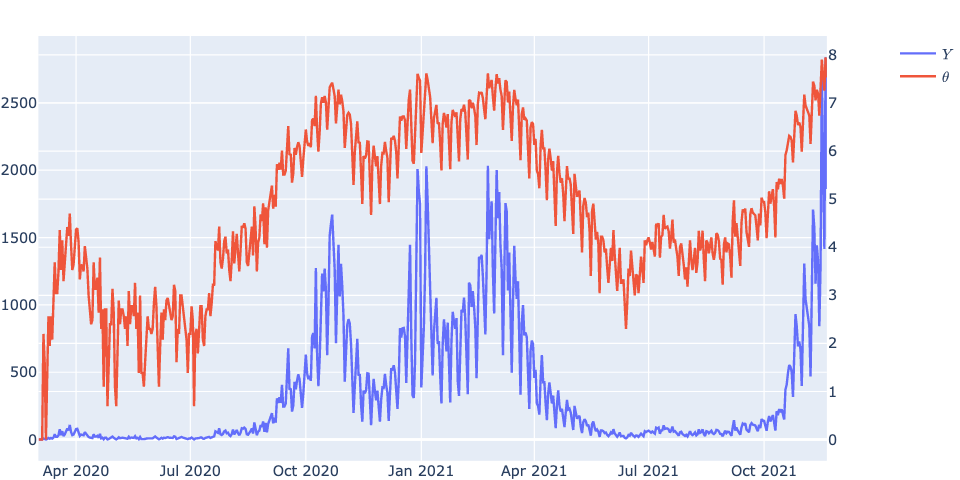
\includegraphics[width=\textwidth]{generated/images/incidence-log-transform.png}
  \end{center}
  \caption{Log transformation of daily incidence}
  \label{fig:incidence-log-transform}
\end{figure}

Moreover, the transformed trends are now 
linear, which implies the exponential growth in the original data.
The likelihood can be finally defined as:

\begin{equation}\label{eq:likelihood-first}
  p( y_c | \theta, \alpha )
\end{equation}

The prior for $\alpha$ was already stated by \eqref{eq:alpha-prior}.
The $\theta$ requires further introspection to choose 
proper distribution.


\section{The analysis of \texorpdfstring{$\theta$}{Lg}}
\label{sec:theta-analysis}

After the transformation, $\theta \in \mathbb{R}$, but, 
as the figure \ref{fig:incidence-log-transform} 
shown, $\theta$ is more homoscedastic random variable, which is 
convenient, because the more homoscedatic 
the r.v. is, the more constant variance 
it has.
This can be verified by first-order detrending/decumulation\footnote{See snippet \ref{snip:theta-diff-plot}} 
of $\theta$, to obtain differences 
$\Delta \theta$, with succesive application of 
$\Delta \theta_t = \theta_{t+1} - \theta_{t}$:

\begin{figure}[H]
  \begin{center}
    \includegraphics[width=11cm]{generated/images/theta-diff.png}
  \end{center}
  \caption{The plot of $\Delta \theta$}
  \label{fig:theta-diff}
\end{figure}

Naturally, we could check normality of the 
whole data, but practically, we will use just 
specific time windows of size $T_w$, in which, the normality of the data will be assumed,
therefore it will be more meaningful to verify normality for those 
windows. In our case, we picked three samples 
of time window $T_w = 50$ as the following figure 
presents\footnote{Created by snippet \ref{snip:theta-diff-sample-windows-plot}}:

\begin{figure}[H]
  \begin{center}
    \includegraphics[width=11cm]{generated/images/theta-diff-sample-windows.png}
  \end{center}
  \caption{The referenced windows for taking samples of $\Delta \theta$}
  \label{fig:theta-sample-windows}
\end{figure}

This means, for the inference of incidence up to time $t$, 
we will assume data only from interval $[t - T_w, t]$, i.e.,
assuming each sample from time period less than
$t - T_w$ is irrelevant.
This will also help to reduce computational complexity.

Let's explore the distribution of those samples 
for confirmation of normality. 
For visual testing of normality, histogram, 
Q-Q and ECDF/CDF plots may be considered. 
Let's start with histograms\footnote{Created by snippet \ref{snip:theta-diff-histogram}}:

\begin{figure}[H]
  \begin{center}
    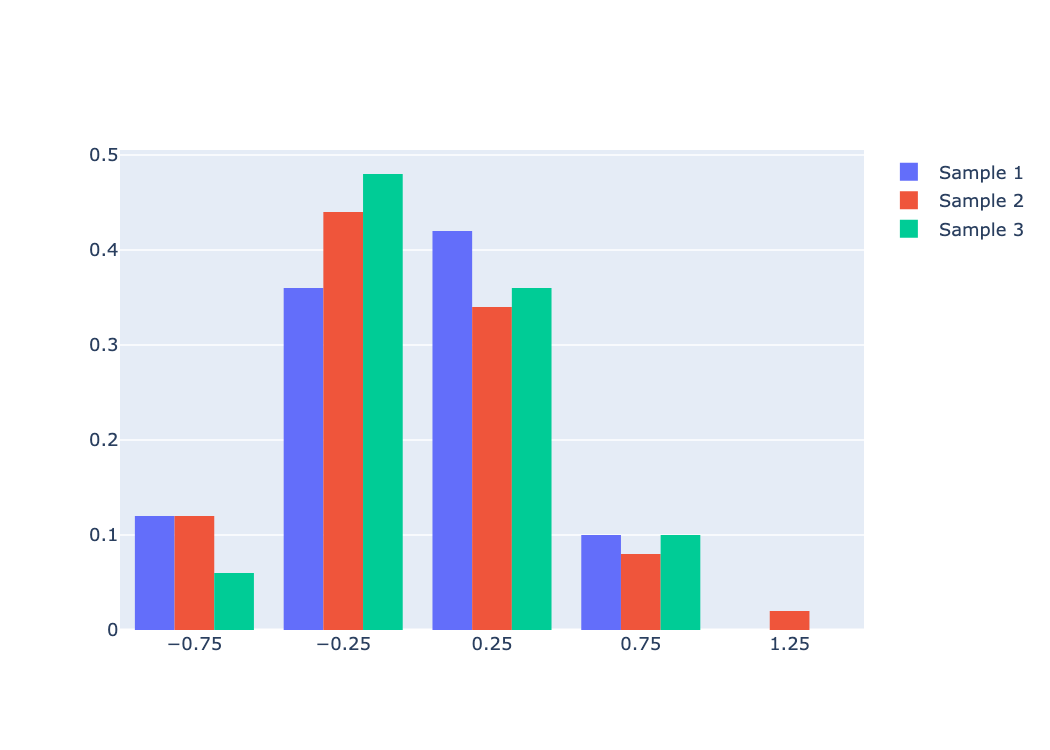
\includegraphics[width=11cm]{generated/images/theta-diff-histogram.png}
  \end{center}
  \caption{The histogram of chosen $\Delta \theta$ samples}
  \label{fig:theta-diff-histogram}
\end{figure}

From the histogram, the normality is not 
very obvious. 
The main pitfall of histogram is the problem 
of choosing the proper bin size, which we may 
think of as some kind of parameter. 
Too narrow bin size means a lot of bins, which 
require a lot of data. 
Too wide bins, on the other hand, ends with 
few bins in the visualisation and we might 
oversee gaps in the data as in our case.
The Q-Q plot is better in this way, because 
it can be assumed as a non-parametric 
visualisation, moreover, we see how all data 
points fit to the normal distribution\footnote{Created by snippet \ref{snip:theta-diff-qq-plot}}:

\begin{figure}[H]
  \begin{center}
    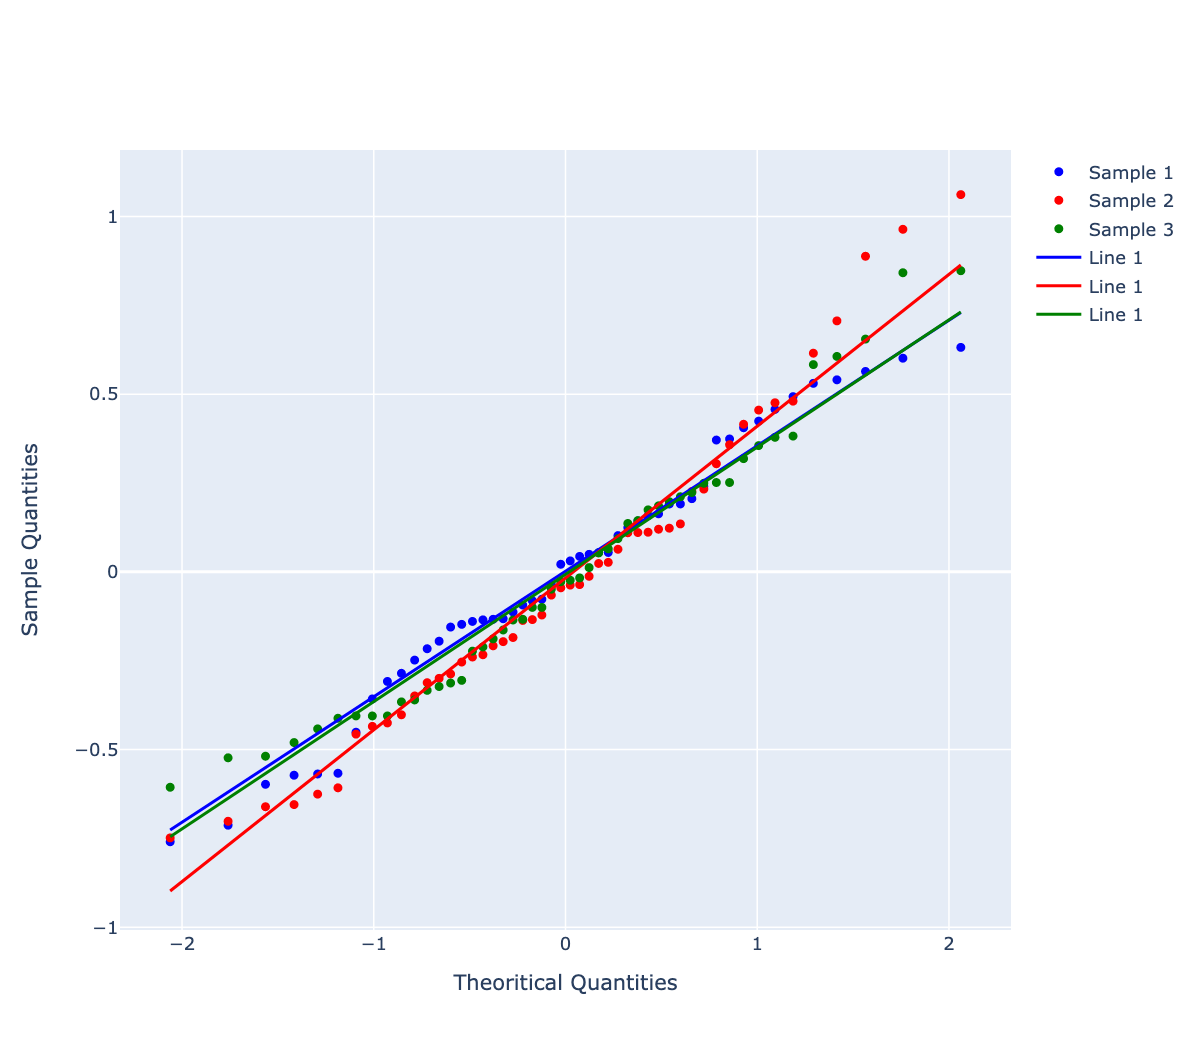
\includegraphics[width=11cm]{generated/images/theta-diff-qq.png}
  \end{center}
  \caption{Quantile-Quantile plot of $\Delta \theta$ samples}
  \label{fig:theta-diff-qq}
\end{figure}


This may finally remind the normally distributed 
data, because closer the points are to the line, 
the more normal distribution is approached in 
the data.

The next plot\footnote{Created by snippet \ref{snip:theta-diff-ecdf-plot}} visualizes the 
\textit{empirical cumulative distribution function}
(ECDF) based on $\Delta \theta$ and CDF for the 
theoretical normal distribution based on 
the summary statistics of $\Delta \theta$:

\begin{figure}[H]
  \begin{center}
    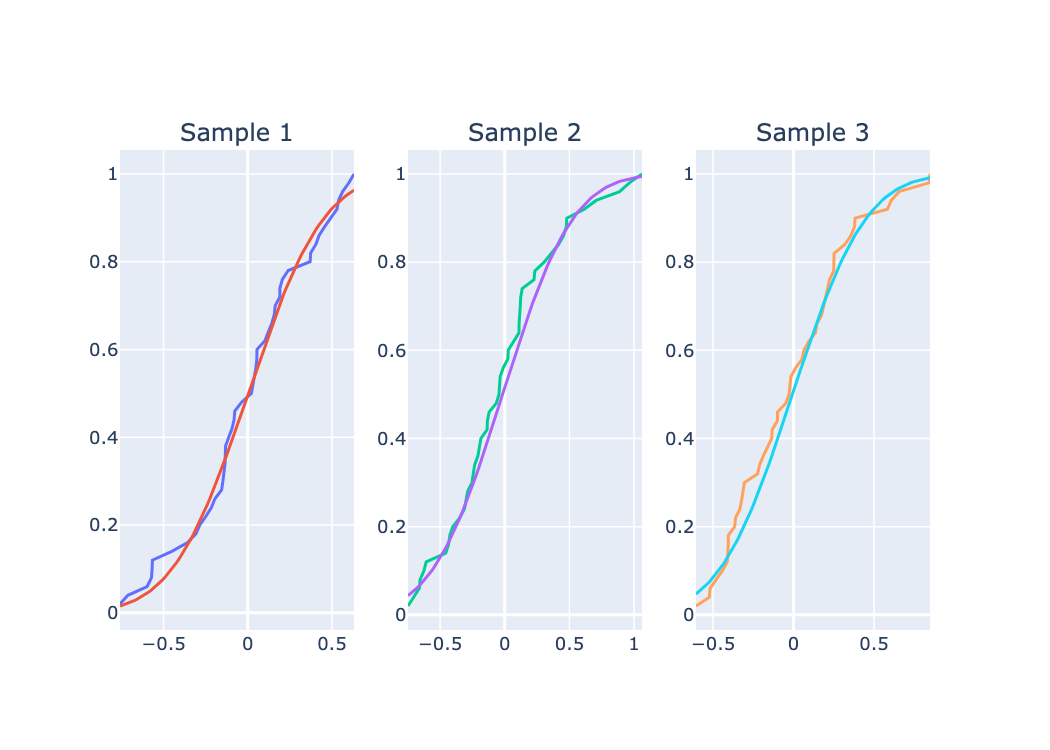
\includegraphics[width=11cm]{generated/images/theta-diff-ecdf.png}
  \end{center}
  \caption{Empirical and theoretical CDFs of $\Delta \theta$ samples}
  \label{fig:theta-diff-ecdf}
\end{figure}

The previous visuals might evoke normally 
distributed data for some individuals, but 
visual check might be misleading, therefore, 
it should not be sufficient for statistical 
modelling. Visual check can be complemented 
also with statistical tests. The 
statistics provides several non-parametric 
normality tests.
In our case, Kolmogorov-Smirnov, Lilliefors and 
Shapiro-Wilk tests were performed.

\input{generated/tables/theta-diff-ks-test}
\input{generated/tables/theta-diff-lilliefors-test}
\input{generated/tables/theta-diff-shapiro-wilk-test}

The strongest result is noted in the 
Lilliefors test, then Shapiro-Wilk test and 
worst result is from Kolmogorov-Smirnov test.
The research of \cite{razali2011} concludes the 
Shapiro-Wilk test to be the most powerful 
normality test and the Kolmogorov-Smirnov test 
to the least powerful (Kolmogorov-Smirnov, 
Shapiro-Wilk, Anderson-Darling and Lilliefors 
tests were compared). 
According to this research and the fact we 
use limiting window $T_w$, the 
assumption about normally distributed $\theta$ 
can be made.
Moreover, as the $\theta$ is actually function of time $\theta(t)$,
we can model its prior as a \textit{Gaussian process}.
Let us introduce theory for Gaussian processes in the
following section, then we will continue
with the prior for $\theta$ in the following section.


\section{Gaussian process}

Gaussian process (GP) is a stochastic process that is used to directly infer
from data over finite set of functions.
Basically, it is a probability distribution over set of
functions which follow \textit{joint (multivariate) Gaussian
distribution} \cite{frigola2015}:

\begin{equation}
    \begin{bmatrix}
      f(x) \\ f(x_\star)
    \end{bmatrix} \sim \text{MN}\left(
    \begin{bmatrix}
      m(x) \\ m(x_\star)
    \end{bmatrix},
    \begin{bmatrix}
      k(x, x) & k(x, x_\star) \\ 
      k(x, x_\star)^\top & k(x_\star, x_\star) \\ 
    \end{bmatrix}
  \right)
\end{equation}

where $f(x)$ is basically internal state 
inferred from the input data (trained model 
in terms of machine learning), and $f(x_\star)$
is a function we want to predict in $x_\star$.

For simplicity, we denote previous as:

\begin{equation}
  f(x) \sim \text{GP} \left( m \left( x \right), k \left( x, x' \right) \right)
\end{equation}

where $m \left( x \right)$ and $k\left( x, x' \right)$ are 
the specifying\footnote{GP is specified only with these two functions} mean and
covariance functions respectively.
For those functions the following apply \cite{rasmussen2004}:

\begin{equation}
\begin{split}
  & m(x) = \mathbb{E} \left[ f(x) \right] \\
  & k \left( x, x' \right) = \mathbb{E} \left[ 
    \left( f \left( x \right) - m \left( x \right) \right)
    \left( f \left( x' \right) - m \left( x' \right) \right)
  \right]
\end{split}
\end{equation}

The mean function, in most cases, is zero function,
mean of the observations, or linear function.

The covariance function is often called 
\textit{kernel function} which is actually \textit{Mercer kernel}, also called 
\textit{positive-definite kernel} \cite{murphy2021}, 
measuring how two inputs $x$ and $x'$ are similar. 
This requires the kernel to be symmetric, i.e., 
$k \left( x, x' \right) = k \left( x', x \right)$.
These kind of function are also called
\textit{smoothing functions/kernels} \cite{martin2016}.

Now lets utilize GP as a prior for $\theta$.

\section{The prior of \texorpdfstring{$\theta$}{Lg}}

The prior of $\theta$ is assumed to be Gaussian process. 
As the GP is probabilistic distribution over the functions,
we need independent variable, in our case, the 
$\theta$ is function of time, such that:

\begin{equation}
  \theta(t) \sim \text{GP}(m, k(t, t^\prime))
\end{equation}

According to the figure \ref{fig:incidence-log-transform}\footnote{Created by snippet \ref{snip:incidence-log-transform-plot}}, 
the linear trend between points should be sufficient, 
therefore let $m$ be defined as:

\begin{equation}
m(t) = b + a t
\end{equation}

where the prior distributions for $a$ and $b$ 
are assumed 
$a \sim N \left( \mu_a, \sigma_a \right)$ and 
$b \sim N \left( \mu_b, \sigma_b \right)$.
Someone may argue why there is no restriction such as
$a \geq 0$, but if $\theta < 0$, then $0 \leq e^{\theta} < 1$, 
which are still valid values for the $\mu$ parameter
of our likelihood.
Basically, we let the $\theta_t$ to move
free in its whole space $\mathbb{R}$, because the
exponential transformation always keeps $\mu \geq 0$.

As a kernel we choose 
the one of the well-known basic kernel \textit{Gaussian kernel}, 
also called \textit{squared exponential kernel} or 
\textit{radial basis function (RBF) kernel} defined as
(for univariate observations):

\begin{equation}
k_{RBF} \left( t, t'; \ell \right) = \exp \left[ -\frac{(t - t')^2}{2\ell^2} \right]
\end{equation}

where $\ell$ is the \textit{length scale} hyperparameter, 
known also as \textit{bandwidth} (denoted $\sigma$ in some literature). 
This hyperparameter is distance which we expect 
differences to matter, in our case\footnote{See snippet \ref{snip:hyperparameters}} $\ell = 7$ as 
we observed weekly seasonality.


\section{Monte Carlo simulation}
\label{sec:monte-carlo}

Simulation itself is relatively old technique for 
solving analytically intractable problems. 
The first such a problem considered is the 
\textit{Buffon's needle problem}\footnote{\url{https://en.wikipedia.org/wiki/Buffon\%27s_needle_problem}} from 1733. 
The probem is defined as probability of the 
needle of length $l$ dropped onto the floor, 
represented by parallel strips of distance 
$d$, crosses the line between two adjacent 
strips.
The analytical solution was discovered in 1777, 
however, the simulation can be done just via 
dropping the needles on the floor and count 
the intersections to calculate probability 
in a frequentistic way.

A huge development in simulation techniques 
naturally came with the development of computers, 
especially during the Los Alamos research 
\cite{metropolis1987}, where 
\textit{Monte Carlo simulation}\footnote{
In fact, the name Monte Carlo refers to the city 
in Monaco, which is famous for its casinos. 
In the casinos, generally, the probability and 
randomness together plays big role, just like in the 
Monte Carlo simulation.
} was invented to 
solve nuclear fission problem.

The whole idea started when Stan Ulam\footnote{\url{https://cs.wikipedia.org/wiki/Stanis\%C5\%82aw_Ulam}} was
trying to compute odds in solitaire.
He tried to solve the problem analytically, but he later
realized the problem could be solved in much simplier way,
just by uniformly sampling layouts of cards in hand and
counting the number of successful games.
This is how the \textit{random sampling} was born.

John von Neumann\footnote{\url{https://cs.wikipedia.org/wiki/John_von_Neumann}}
was interested in the Stan's idea. He saw a big potential for
solving untractable problems in physics.
Unfortunatelly, in physics, there are many problems where
we know some distributions in theory but they are difficult
to sample from, so he later invented 
\textit{rejection sampling} \cite{beichl2000}, which 
was a foundation for the future development of 
Monte Carlo techniques.

Monte Carlo methods can be used for various 
purposes, mostly used for integration and
optimizations problems,
for example, in the Bayesian inference is used for \cite{andrieu2003}:

\begin{itemize}
  \item \textit{Normalization} - computing posterior $p(X | Y)$ from:
    \begin{equation}
      p(X | Y) = \frac{p(Y | X) p(X)}{\int_{\mathcal{X}} p(Y | X^\prime) p(X^\prime) dX^\prime}
    \end{equation} \\
    where the denominator is the normalizing constant $\eta$ which is usually intractable.
  \item \textit{Maginalization} - computing marginal probability $p(Y)$ from the joint distribution $p(X, Y)$:
    \begin{equation}
      p(Y) = \int_{\mathcal{X}} p(X, Y) dx
    \end{equation} \\
    This is basically just a subtask of the normalization mentioned before.
  \item \textit{Expectation} - to calculate expected value as in \eqref{eq:random-sampling-expectation}
\end{itemize}


\subsection{Random sampling}

Let's imagine we have a random variable 
$x \in \mathcal{X}$ distributed according to 
$p$ and we are interested in its expected 
value $\mathbb{E}_p$. 
The usual approach would be:

\begin{equation}\label{eq:random-sampling-expectation}
  \mathbb{E}_{p}\left[ f(x) \right] = \int_{\mathcal{X}} p \left( x \right) f \left( x \right) dx
\end{equation}

But in many cases, the $p$ is not directly 
observable, as we usually do not have all the 
possible data.
The Monte Carlo may approach this value by 
generating $n$ independent identically distributed 
random samples $x_i$ (if sampling from $f$ is 
possible) from domain $\mathcal{X}$ to form a 
sample mean of that unknown quantity:

\begin{equation}
  \hat{\mu}_n = \frac{1}{n} \sum_{i=1}^{n} f_{x_i}
\end{equation}

According to the unknown quantity above, this 
is its \textit{unbiased Monte Carlo estimator}, i.e. 
estimator of the expected value. 
As $n \to \infty$, from the law of large numbers, 
we can state 
$\hat{\mu}_{\infty} = \mathbb{E}_{\pi}\left[ f(x) \right]$, 
therefore for very large $n$ it holds 
$\hat{\mu}_n \approx \mathbb{E}_{\pi}\left[ f(x) \right]$.

In this approach, the samples are trully 
random meaning independent of each other, 
hence the name \textit{random sampling}.
The main pitfall of random sampling is its 
computationally inefficiency, i.e., we 
need $n$ to be a very large number to be 
sure the samples sufficiently cover 
$\mathcal{X}$, even for highly unprobable
values of $x_i$, i.e., $\pi(x_i) \approx 0$.


\subsection{Rejection sampling}
\label{sec:rejection-sampling}

In rejection sampling, the basic assumption is we have \textit{target
probability distribution} $f$ for which we want to estimate
some quantity. Unfortunatelly, we are not able to sample
from $f$ or the sampling is somehow complicated.
Rejection sampling overcoming this by sampling
from other, related to the $f$ and easy to sample from, 
\textit{proposal distribution} $g$.
The algorithm proceeds as follows \cite{beichl2000}:

\begin{enumerate}
  \item Sample proposal $x \sim g(x)$
  \item Generate $u \sim \text{Uniform}(0, 1)$
  \item If $u < \frac{f(x)}{M g(x)}$ accept $x$
  \item Go to step 1
\end{enumerate}

In the first step, the sample $x$ from a proposal
distribution $g$ is generated.
Then $u$ is randomly chosen such that $u \in [0, 1)$.
As the condition in \eqref{eq:rejection-sampling-cond}
must be kept, then $\frac{f(x)}{M g(x)} \leq 1$.
The ratio $\frac{f(x)}{M g(x)}$ closer to $1$
means the $x$ was generated from higher density
region, rather than, when this ratio is closer 
to $0$.
Basically, higher the ratio is the more likely
we accept $x$, and after sufficient amount of 
steps, or accepted samples, the algorithm might 
be terminated.
The acceptation in this algorithm is related 
with the term \textit{acceptance rate}, which is
the ratio of number of accepted samples and 
number of total samples generated.

The algorithm depends on a very limiting condition:

\begin{equation}\label{eq:rejection-sampling-cond}
  M \geq \frac{f(x)}{g(x)}, \forall x
\end{equation}

This means we have to choose sufficiently large $M$
such that we are ensured the $M g(x)$ for every $x$
creates envelope around whole $f$.
However, if we pick $M$ too high,
we will reject most of the samples, i.e., we will 
achieve very low acceptance rate and
the simulation will be computationally inefficient.

The condition \eqref{eq:rejection-sampling-cond},
and therefore the problem with acceptance rate,
may be overcomed with employment of some type
of memory.


\section{Markov Chain Monte Carlo}

\textit{Markov Chain Monte Carlo} (MCMC) is a class of 
algorithms solving problem with sampling from a 
\textit{target probability distribution} $f$ in more 
efficient way than random sampling mentioned before. 
Basic principle is to walk through 
distribution, similarly as random sampling 
does, but we also utilize the previously
generated samples.
These samples are forming a sequence
assuming Markov property, hence the
name \textit{Markov chain}.
This Markov chain can be assumed as a some kind of
short-term memory.


\subsection{Metropolis algorithm}

The algorithm is named after his inventor, 
Nicholas Metropolis\footnote{\url{https://en.wikipedia.org/wiki/Nicholas_Metropolis}}, and is very first Monte 
Carlo algorithm utilizing Markov chains 
\cite{metropolis1953}.
Lets imagine, we are interested in theoretical 
probability distribution $f(x)$ of 
some parameter $x$, which is not easily tractable 
(same as in the case of rejection sampling).
The idea is to gradually generate the 
$x^\prime$ parameter into the sequence 
forming Markov chain.
The generation is done with a proposal distribution 
$g(x^\prime | x_{i})$ conditionally dependent on the last sample
$x_{i}$ in the forming Markov chain\footnote{To be more specific, since the $g$ is conditionally dependent only on the last sample, it is so-called first-order Markov chain} $X_{0:i}$.
Assume input $x_0$ and $i = 0$, then the algorithm process itself 
might be summarized in the following steps:

\begin{enumerate}
  \item Generate proposal $x^\prime \sim g(x^\prime | x_{i})$
  \item Compute $\alpha$ according to \eqref{eq:metropolis-alpha}
  \item Generate $u \sim \text{Uniform}(0, 1)$
  \item Set $x_{i+1} \leftarrow \begin{cases}
    x^\prime, & \text{ if } u \leq \alpha,\\
    x_{i}, & \text{ ow.}
    \end{cases}
    $
  \item Set $i \leftarrow i + 1$ and go to \textit{step 1}
\end{enumerate}

In the first step, the parameter proposal $x^\prime$ is generated from proposal distribution $g$.
The second step assumes computation of the \textit{acceptance probability} $\alpha$:

\begin{equation}\label{eq:metropolis-alpha}
  \alpha = \min \left(1, \frac{f(x^\prime)}{f(x_{i})}\right)
\end{equation}

The ratio $\frac{f(x^\prime)}{f(x_{i})}$ expresses 
how many times $x^\prime$ is more probable than $x_{i}$.
This probability is then compared with uniformly generated $u \in [0, 1)$. 
Note the similarity with rejection sampling defined in 
\autoref{sec:rejection-sampling}.
This may look a little bit cumbersome, 
because of possibility of accepting $x^\prime$ with 
lower probability than $x_{i-1}$, but the 
whole idea of acceptance probability is to let 
explore further areas of state space to prevent 
stuck in local minimum. Basically, the 
probability of transition into particular state is
proportional to the probability of that state, i.e.,
the states with higher probabilities are preferred.

For the initial state 
$x_0$, we usually put our initial prior, 
which affects the speed of convergence - 
the more accurate prior is the faster the 
convergence is.
After sufficient amount of steps, the Markov 
chain should reach the stationary target 
distribution $f(x)$,

One of the primary pitfalls of the Metropolis algorithm is
its unability in using asymmetric proposal distributions.
This issue is solved by Hasting's modification.
% These number of 
% sufficient steps defines \textit{burnin period} 
% referencing the samples being discarded. This 
% is happening because it usually takes a while 
% until the parameters converge to form 
% a stationary distribution. It primarily 
% depends on the choice of prior as was mentioned. 
% Basically we take the last $n$ samples of the 
% chain to represent samples from 
% the posterior distribution.


\subsection{Metropolis-Hastings algorithm}

Metropolis-Hastings algorithm is a generalization
of the Metropolis algorithm allowing to sample from
asymmetric proposal distributions.
This modification was first introduced by 
Wilfred K. Hastings in 1970, only by 
using the following acceptance probability $\alpha$:

\begin{equation}\label{eq:metropolis-hastings-alpha}
  \alpha = \min \left(1, \frac{f(x^{\prime})}{f(x_{i})} \frac{g(x_{i} | x^{\prime})}{g(x^{\prime} | x_{i})}\right)  
\end{equation}

The difference lies only in adding multiplication
by the ratio $\frac{g(x_{i} | x^{\prime})}{g(x^{\prime} | x_{i})}$
which is originally derived from the detailed 
balance principle \cite[Chapter 11]{owen2013}:

\begin{equation}
  p(x^\prime | x) p(x) = p(x | x^\prime) p(x^\prime)
\end{equation}

Although the Metropolis algorithm was generalized to
use asymmetric proposals, it is still quite inefficient
in the exploring state space, especially for
multidimensional problems, because of its 
randomness proposal, moreover, highly dependent 
on parametrization.


\subsection{Boltzmann factor}
\label{sec:boltzmann-factor}

In many cases, the ratio of 
two probabilities (as was seen in 
\eqref{eq:metropolis-alpha} and \eqref{eq:metropolis-hastings-alpha}) is not
computationally very feasible because of possibility of dividision 
with very small numbers (even $0$) or infinity values.
Therefore, for practical purposes, the physical analogy with 
\textit{Boltzmann distribution} is being used \cite{murphy2021}.
The Boltzmann distribution represents a probability of 
certain state $x$ of physical system as:

\begin{equation}\label{eq:boltzmann-factor-prop}
  p(x) \propto \exp \left( -\frac{E(x)}{kT} \right)
\end{equation}

where $E(x)$ is energy of $x$, $T$ is 
temperature and $k$ is Boltzmann's constant\footnote{\url{https://en.wikipedia.org/wiki/Boltzmann_constant}}.
Since $k$ is always constant and we do not need 
to simulate exact physical result of particles, 
we getting rid of $k$ and proportionality.
$T$ is usually used in the \textit{simulated annealing} where we
decrease $T$ gradually with time (more on this in \cite[Chapter 8]{murphy2021}),
however, in this case we do not employ that, i.e., assuming $T = 1$, then:

\begin{equation}\label{eq:boltzmann-factor-prob}
  p(x) = \exp \left( -E(x) \right)
\end{equation}

And analogically:

\begin{equation}\label{eq:boltzmann-factor-neg-log}
  E(x) = -\log p(x)
\end{equation}

The basically states, the lower energy $E(x)$ of $x$ the higher probability of $x$.
In statistics, $E$ is, in this case, called \textit{negative log probability}.
Now we can derive the formula for the ratio of probabilities:

\begin{equation}
  \frac{p(x)}{p(y)} = \exp \left( -(E(x) - E(y)) \right) = \exp \left( E(y) - E(x) \right)
\end{equation}

For example, the acceptance probability \eqref{eq:metropolis-alpha} for Metropolis can be rewritten:

\begin{equation}
  \begin{split}
    \alpha &= \min \left(
    1, 
    \exp\left( 
      E(x_{i}) - E(x^\prime)
    \right) 
  \right) \\
  & = \min \left(
    1, 
    \exp\left( 
      \log f(x^\prime) - \log f(x_{i})
    \right) 
  \right)
  \end{split}
\end{equation}

Similarly for the ratio in acceptance probability \eqref{eq:metropolis-hastings-alpha} of Metropolis–Hastings:

\begin{equation}
  \exp \left( \log f(x_{i}) + \log g(x^{\prime} | x_{i}) - \log f(x^\prime) - \log g(x_{i} | x^{\prime}) \right)
\end{equation}

% \begin{equation}\label{eq:metropolis-hastings-alpha}
%   \alpha = min\left(1, \frac{f(x^{\prime})}{f(x_{i})} \frac{g(x_{i} | x^{\prime})}{g(x^{\prime} | x_{i})}\right)  
% \end{equation}

\subsection{Hamiltonian Monte Carlo}

\textit{Hamiltonian Monte Carlo} (HMC) is another Metropolis-Hastings 
based algorithm, but it utilizes physical analogy to 
generate proposals more efficiently as the gradient 
of proposal distribution is available \cite{betancourt2018}.

It started with Hybrid Monte Carlo paper \cite{duane1987}, 
which utilized Monte Carlo to understand the structure 
of atoms. 
Radford Neal laterly recognized the potential of 
this method during his focus on Bayesian neural networks 
within his doctoral thesis \cite{neal1995}. 
\cite{mackay2003} started to use 
term \textit{Hamiltonian Monte Carlo} under which this 
method is known to this day.
Neal, again, did a big review of HMC \cite{neal2011}.
But for wider use, HMC had to 
wait to advent of highly efficient 
computational software allowing its practical usage.

In Hamiltonian dynamics, state is characterized by the
\textit{position vector} $x$ and the \textit{momentum vector} $p$,
both are $d$-dimensional, hence $2d$-dimensional state.
We usually measure total energy in the system by the function of
the state $H(x, p)$ called \textit{Hamiltonian}.
The Hamilton’s equations describe how position $x$ and
$p$ change according to time $t$ by 
the partial derivatives \cite{neal2011}:

\begin{equation}
  \frac{\partial x_i}{\partial t} = \frac{\partial H}{\partial p_i}
\end{equation}

\begin{equation}
  \frac{\partial p_i}{\partial t} = - \frac{\partial H}{\partial x_i}
\end{equation}

where $i = 1, \dots, d$ is the dimension.
The Hamiltonian $H$ can be tought as a total energy in whole system,
i.e., sum of \textit{potential energy} $U$ and \textit{kinetic energy} $K$:

\begin{equation}
  H(x, p) = U(x) + K(p)
\end{equation}

The $U$ corresponds to the equation 
\ref{eq:boltzmann-factor-neg-log}, i.e., is assumed as negative log 
probability density of posterior $f(x)$ we want to sample from:

\begin{equation}
  U(x) = -\log f(x)
\end{equation}

The lower the probability $f(x)$ is, the higher 
energy $U(x)$ we obtain. 
Then we can rewritte partial derivative for momentum $p$ as:

\begin{equation}
  \frac{\partial p_i}{\partial t} = - \frac{\partial U}{\partial x_i}
\end{equation}

Kinetic energy $K(p)$ in 
multidimensional fashion is, according to physics, calculated as:

\begin{equation}
  K(p) = \frac{p^{\top} M^{-1} p}{2}
\end{equation}

where $M$ is symmetric, positive-definite mass 
matrix (often scalar-scaled identity matrix \cite{neal2011}).
With previous knowledge, the Hamiltonian 
equation for position (parameters) $x$ can be rewritten as:

\begin{equation}
  \frac{\partial x_i}{\partial t} = \frac{p_i}{m_i}
\end{equation}

The discretization is a necessary step in terms of 
solving Hamiltonian equations by computers.
There are several methods of discretization, where 
the best-known is probably \textit{Euler's method}\footnote{\url{https://en.wikipedia.org/wiki/Euler_method}}.
Unfortunatelly, in the case of Hamiltonian equations, 
Euler method is not performing too accurate 
\cite[Chapter 5]{neal2011}.
As the one partial equation is dependent on another,
HMC approaches derivatives with the
\textit{leapfrog method} (or \textit{leapfrog intergration}) which 
is simple for implementation \cite{betancourt2018}, but very efficient.
The discretized equations approaches the integration 
by interleaving 1/2 step $\epsilon$ to update internal
HMC state (vectors $x$ and $p$) as follows:

\begin{equation}
  p_i \left(t + \frac{\epsilon}{2} \right) = p_i(t) - \frac{\epsilon}{2} \frac{\partial U}{\partial x_i} (x(t))
\end{equation}

\begin{equation}
  x_i(t + \epsilon) = x_i(t) + \epsilon \frac{p_i \left(t + \frac{\epsilon}{2} \right)}{m_i}
\end{equation}

\begin{equation}
  p_i(t + \epsilon) = p_i \left( t + \frac{\epsilon}{2} \right) - \frac{\epsilon}{2} \frac{\partial U}{\partial x_i} \left( x \left( t + \epsilon \right) \right)
\end{equation}

These equations are applied $L$ times, where $L$ is number 
of leapfrog steps. 
As $\epsilon$ is a size of step, then $x(t + L \epsilon)$ is
the final position we obtain after leapfrog integration.
In the end of the step, the HMC approaches similarly as
Metropolis algorithm, except the acceptance probability $\alpha$
is computed from the Hamiltonian $H$, employing 
Boltzmann factor (\ref{eq:boltzmann-factor-prop}):

\begin{equation}
  \alpha = \min \left( 1, \exp \left( H(x(t), p(t)) - H(x(t + L \epsilon), p(t + L \epsilon)) \right) \right)
\end{equation}

% Then we are just applying Metropolis algorithm

% To transform energy into probability, HMC utilizes Boltzmann factor,
% i.e., equation , the probability
% of particular state $x$ and $p$ can be expressed (with $kT = 1$) as:

% \begin{equation}
%   p(x) = \frac{1}{\eta} \exp \left( -E(x) \right)
% \end{equation}

% with $\eta$ as a normalizing constant.
% Now we can put Hamiltonian $H$ to obtain:

% \begin{equation}
%   p(x, p) = \frac{1}{\eta} \exp \left( -H(x, p) \right) = \frac{1}{\eta} \exp \left( -U(x) \right) \exp \left( -K(p) \right)
% \end{equation}

Although the algorithm is much more complex than
Metropolis-Hastings algorithm, i.e., the one iteration
of HMC takes longer than MH, HMC usually reaches stationary 
distribution after fewer iterations as the proposal is
moving according to the gradient, and not randomly as 
in the case of MH.


\subsection{No U-Turn Sampler}
\label{sec:nuts}

The \textit{No U-Turn Sampler} (NUTS) was first introduced in 
paper \cite{hoffman2011}. In HMC, parameters $L$ and $\epsilon$ 
have to be tuned. This might cause several problems when 
finding proper values for demanding convergence.
According to \cite{betancourt2018}, if the integration 
trajectory is too short (i.e., low $L\epsilon$),
we are not taking full advantage of HMC and rather
approach MH, on the other hand, of it is too long (i.e., too high $L$),
the algorithm is computationally inefficient.

\textbf{TODO}

For additional information and nice visualisations of 
MH, HMC and NUTS, please see \cite{mcelreath2017}.

\section{PyMC3}

PyMC3 is probabilistic programming tool, more specifically, 
it is a Python package capable of Bayesian statistical 
inference using both stochastic and deterministic algorithms. 
The features include variety of MCMC and variational inference algorithms,
Gaussian processes, advanced plotting
(using ArViz library) and more\footnote{\url{https://docs.pymc.io/en/v3/}}.

PyMC began to be developed in 2003 with idea
bringing Metropolis–Hastings samplers closer to 
the applied scientists.
First public version was released in 2005,
after few year, in 2011, the development team
started to solve how to implement gradient-based MCMC samplers
to boost up the performance.
These were brought into PyMC in version 3
in 2015 when first alpha was released, and
the first official release of PyMC3 was in 2017.

The PyMC3 is built upon a Theano\footnote{currently fork of 
Theano called Aesara, Theano is not developed anymore},
which basically allows descriptive modelling 
of mathematical operations.
These are then optimized and transformed,
without much of the user's effort, to 
the low level instructions to support efficient 
processing by CPU(s) or GPU(s), which is convenient 
especially for operations with large arrays.
Similar principle can be seen also in Tensorflow 
\cite{tf} or PyTorch \cite{pytorch}.
This is kind of similar to query planning and execution
in big data processing, where the user desribes what
he wants, but usually does not tell the system how 
to achieve it.

Another alternatives to PyMC3 are, for example,
TensorFlow Probability \cite{tfp}, Pyro \cite{pyro} and
Stan\footnote{The name gives honour to Stan Ulam, father of MC, as mentioned in \autoref{sec:monte-carlo}} \cite{stanmc}
(and its Python alternative PyStan).
The reason for choosing PyMC3 over others is its
easy Python integration, high-level of abstraction,
and wide community of users.


\section{The probabilistic model revisited}

Let us recall the chosen probabilistic model of incidence.
The likelihood is given by the \textit{negative binomial distribution}:

\begin{equation}
  c \sim \text{NegBin} (\mu=exp(\theta), \alpha)
\end{equation}

which is dependent on $\theta$ and $\alpha$ variables distributed as:

\begin{equation}
  \alpha \sim \text{Exponential} (\lambda_\alpha)
\end{equation}

\begin{equation}
  \theta(t) \sim GP(m=b + at, k=k_{RBF} \left( t, t'; \ell \right))
\end{equation}

The $\theta$ is dependent on the selection of 
coefficient $a$ and $b$ for linear trend, which are 
given by Gaussians:

\begin{equation}
  \begin{split}
    a \sim N(\mu_a, \sigma_a) \\
    b \sim N(\mu_b, \sigma_b)
  \end{split}
\end{equation}

In the model $\mu_a$, $\mu_b$, $\sigma_a$, $\sigma_b$, 
$\lambda_\alpha$ and $\ell$ can be 
considered hyperparameters, which are tunned manually.

Lets apply the previous to the Bayesian theorem.
To recall \eqref{eq:bayes-theorem-customized}:

\begin{equation}
  p( X | Y_c, Z ) = \eta^{-1} p( Y_c | X ) p(X | Z)
\end{equation}

The latent state $X$ is a set of parameters we would like
to infer, in our case $X = (\theta, \alpha, a, b)$.
$Z$ is a set of hyperparameters tuned manually 
$Z = (\lambda_\alpha, \ell, \mu_a, \mu_b, \sigma_a, \sigma_b)$.

Therefore our posterior is given by:

\begin{equation}
  p \left( \theta, \alpha, a, b | Y_c; \lambda_\alpha, \ell, \mu_a, \mu_b, \sigma_a, \sigma_b \right)
\end{equation}

which is proportional to:

\begin{equation}\label{eq:inc-model-joint-expanded}
   p( Y_c | \theta, \alpha ) p( \alpha | \lambda_\alpha ) p ( \theta | a, b, \ell ) p ( a | \mu_a, \sigma_a ) p ( b | \mu_b, \sigma_b )
\end{equation}

This definitely would not have an easy analytical solution,
as we have to integrate over all
$\theta$, $\alpha$, $a$ and $b$ to obtain normalization constant,
so lets employ MCMC theory through PyMC3 computation to
help us to infer $X$.


\section{The inference of incidence}
\label{sec:inference-of-incidence}

We are now getting to the core of the problem itself, 
the inference of unknown 
parameters $X$ via PyMC3. Naturally, PyMC3 have to build 
its own internal representation of a model.
The internal representation looks like
a \textit{directed acyclic graph} (DAG), which
is basically a \textit{Bayesian network}:

\begin{figure}[H]
  \begin{center}
    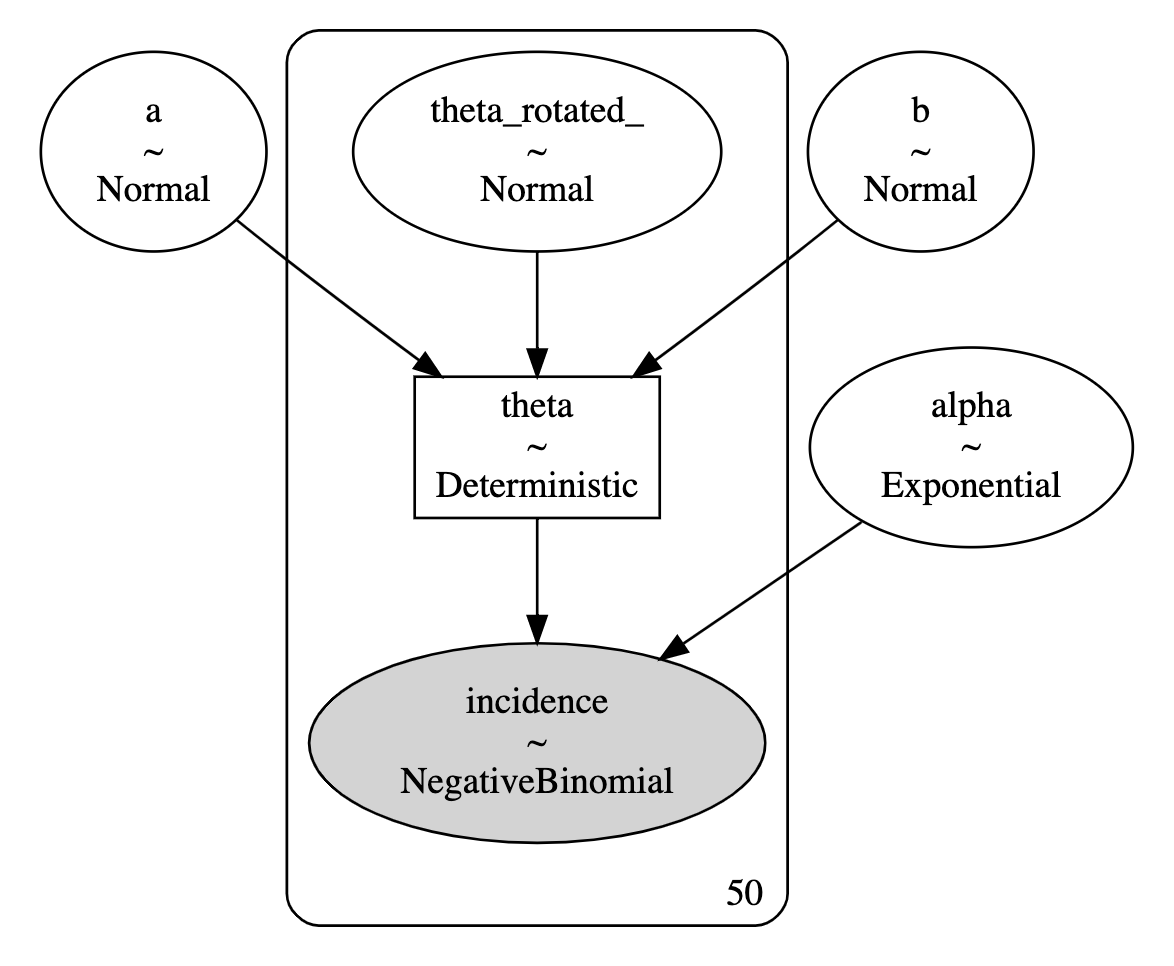
\includegraphics[width=8cm]{static/images/inc-model-graphviz.png}
  \end{center}
  \caption{Internal PyMC3 DAG representation of our incidence model}
  \label{fig:inc-model-graphviz}
\end{figure}

In the figure \ref{fig:inc-model-graphviz}\footnote{Created by snippet \ref{snip:inc-model-graphviz}},
we can see how PyMC3 represents our particular incidence model (given by snippet \ref{snip:inc-model-build-func}),
where the shapes represents each particular distribution.
The highlighted shape is a likelihood and the outlined 
shapes represent priors, similarly as our theoretical 
model \ref{eq:inc-model-joint-expanded}.
The only minor discrepancy might be seen in PyMC3's representation of $\theta$.
This is given by the nature of $\theta$ as a Gaussian process, as it is 
basically multidimensional normal distribution,
and PyMC3 uses\footnote{See \url{https://github.com/pymc-devs/pymc/blob/main/pymc/gp/gp.py\#L303}} rotating by \textit{Cholesky 
factor} \cite[Chapter 7]{murphy2021}.
In our case, the dimensionality of $\theta$ is equal to 
the size of incidence window $T_w$.

To approximate incidence properly, we need to tune up model for
as much specific cases as possible. Ideally, we should try to approximate
whole incidence upon all the data, however, it will be very laborious 
due to the dimensionality of the data.

As was mentioned in \autoref{sec:theta-analysis} we will 
estimate incidence for samples of size $T_w$ only instead the whole time series.
In this particular case, as we have to tune the model, 
those samples should represent various heterogeneous cases to ensure 
robustness of the model.
For this reason, we picked the following samples for incidence fitting:

\begin{enumerate}
  \item Noisy incidence as in \ref{fig:dev-incidence-1}\footnote{Created by snippet \ref{snip:inc-model-sample-incidence-1}}:
  \begin{figure}[H]
    \begin{center}
      \includegraphics[width=9cm]{generated/images/inc-model-sample-incidence-1.png}
    \end{center}
    \caption{Sample 1 for the incidence inference tuning}
    \label{fig:dev-incidence-1}
  \end{figure}
  \item Low (almost zero) incidence (\ref{fig:dev-incidence-2}\footnote{Created by snippet \ref{snip:inc-model-sample-incidence-2}})
  \item Regular growing incidence (\ref{fig:dev-incidence-3}\footnote{Created by snippet \ref{snip:inc-model-sample-incidence-3}})
\end{enumerate}


\subsection{Sampling}

For sampling the posterior distribution we use NUTS, mentioned
in \autoref{sec:nuts}, because of its good performance 
in multidimensional problems.
In PyMC3, the NUTS sampler has several options
to tune for better performance\footnote{See official documentation \url{https://docs.pymc.io/en/v3/api/inference.html}}, but for our case, the
basic settings are sufficient.

Now we are ready for sampling.
Usually, in MCMC inference, we run several independent
Markov chains in parallel.
This is because sometimes the convergence may not be 
successful and we are not able to recognize that.
If we run multiple simulations in parallel,
we can compare results with each other.

After sampling 4 chains, we obtain the following posterior
distribution of $X$:

\begin{figure}[H]
  \begin{center}
    \includegraphics[width=10cm]{generated/images/inc-model-params-trace-1.png}
  \end{center}
  \caption{Posterior trace of parameters $X$ for sample 1}
  \label{fig:params-trace-1}
\end{figure}

On the left side, in the figure \ref{fig:params-trace-1}\footnote{Created by snippet \ref{snip:inc-model-sampling-trace-plot-1}},
we see results for each of the parameters 
$\theta$, $\alpha$, $a$ and $b$ as rows.
On the left side of the figure, we see how each 
particular chain for each variable performed in 
comparison with other chains of that variable.
On the right side, we see the chain of 500 samples 
we desired (samples from burnin period are discarded) for 
each variable.
Note the dimensionality of $\theta$ makes this 
figure a little bit unclear.
For this purposes we can plot the posterior of 
the Gaussian process in a separated plot\footnote{Created by snippet \ref{snip:inc-model-theta-posterior-1}}:

\begin{figure}[H]
  \begin{center}
    \includegraphics[width=10cm]{generated/images/inc-model-theta-posterior-1.png}
  \end{center}
  \caption{Posterior of $\theta$ for sample 1}
  \label{fig:theta-posterior-1}
\end{figure}

The figure \ref{fig:theta-posterior-1} may somehow remind
the original data (actually it should be the logarithm of the incidence mean).
To check if our model performed well, we usually 
need to plot something we can compare. In the case of
Bayesian inference, we can use \textit{posterior predictive check}.


\section{Posterior predictive check}

\textit{Posterior predictive check} (PPC) can be characterized as a replication
of the original dataset from the inferred data. 
Basically, we reverse the inference algorithm,
i.e., take inferred parameters and utilize them to generate
approximation of the observed data \cite{davidson-pilon2015}.
This allows us to check the discrepancies between that approximation
and observed data.

The following plots present capability of fitting the observed
incidence by the incidence model presented before. The first plot
is valid for the first sample (\ref{fig:dev-incidence-1}) of incidence observations defined in \autoref{sec:inference-of-incidence}.
To recall, the first sample represents noisy 
observations (PPC in figure \ref{fig:incidence-posterior-1}\footnote{Created by snippet \ref{snip:inc-model-ppc-plot-1}}):

\begin{figure}[H]
  \centering
  \includegraphics[width=11cm]{generated/images/inc-model-ppc-plot-1.png}
  \caption{Posterior predictive of $\hat{c}$ for sample 1}
  \label{fig:incidence-posterior-1}
\end{figure}

The second sample (\ref{fig:dev-incidence-2}) represents low (almost zero) 
incidence (PPC in figure \ref{fig:incidence-posterior-2}\footnote{Created by snippet \ref{snip:inc-model-ppc-plot-2}}):

\begin{figure}[H]
  \centering
  \includegraphics[width=10cm]{generated/images/inc-model-ppc-plot-2.png}
  \caption{Posterior predictive of $\hat{c}$ for sample 2}
  \label{fig:incidence-posterior-2}
\end{figure}

And finally, the third sample (\ref{fig:dev-incidence-3}) is for
regularly growing
incidence (PPC in figure \ref{fig:incidence-posterior-3}\footnote{Created by snippet \ref{snip:inc-model-ppc-plot-3}}):

\begin{figure}[H]
  \centering
  \includegraphics[width=10cm]{generated/images/inc-model-ppc-plot-3.png}
  \caption{Posterior predictive of $\hat{c}$ for sample 3}
  \label{fig:incidence-posterior-3}
\end{figure}


\chapter{The risk estimation}

In the previous chapter, we achieved a proper settings
to estimate incidence $\hat{c}$ via \textit{smoothening}
observated noisy incidence $Y_c$.
Now we have to employ previously established epimiological theory,
and utilize inferred incidence $\hat{c}$ to compute the risk.
To compute risk, we need to know prevalence $I$, which we 
will approximate from $\hat{c}$.
The necessary theory was established in \autoref{chap:epidemiological-prerequisites} and \autoref{sec:data-based-approach}.


\section{Prevalence estimation}

This section shows how to obtain prevalence
estimation $\hat{I}$ from $\hat{c}$ and how those two relates to each other.
To be sure, our model works well, we need to somehow 
validate the output values, however, we do not know 
true prevalence because it is not available information within the data we use.

Therefore, we will choose another approach.
We will generate synthetic data from an artificial model
with known parameters.
This artifical model should take $\mathcal{R}_e$ as
a parameter as we want to generate $\mathcal{R}_e$ on our own.
Moreover, this model should be able to produce 
also $I$ to compare.
As this artificial model, we will use SIR model because 
of its large parametrization options, but 
we have to modify it to allow using 
$\mathcal{R}_e$ as a parameter.

Lets take equation \ref{eq:sir-model-incidence} and discretize it by the Euler's method:

\begin{equation}
  \label{eq:risk-model-incidence}
  c = \beta_t I_{t-1} \frac{S_{t-1}}{N}
\end{equation}

Also discretize the equation 
\eqref{eq:sir-effective-reproduction-number} for $\mathcal{R}_e(t)$ for SIR model:

\begin{equation}\label{eq:risk-model-rt}
\mathcal{R}_{et} = \mathcal{R}_0 \frac{S_{t-1}}{N} = \frac{\beta}{\gamma} \frac{S_{t-1}}{N}
\end{equation}

To incorporate $\mathcal{R}_{et}$ we will assume $\beta$ changes with time, hence $\beta_t$:

\begin{equation}
\beta_t = \frac{\gamma_t N \mathcal{R}_{et}}{S_{t-1}}
\end{equation}

The only thing remains is to solve $\gamma$. According to \cite{ma2019},
the average mean time of infection can be assumed $\gamma^{-1}$.
For simplicity, we will use expected value of serial interval:

\begin{equation}
  \gamma = \frac{1}{\mathbb{E}[\omega]}
\end{equation}

Substituting into incidence equation \eqref{eq:risk-model-incidence} we get:

\begin{equation}
  c = \gamma \mathcal{R}_{et} I_{t-1} = \frac{\mathcal{R}_{et} I_{t-1}}{\mathbb{E}[\omega]}
\end{equation}

In our case, the following function was used to generate 
artifical $\mathcal{R}_{e}$:

\begin{equation}
  \mathcal{R}_{e}(t) = 1 + \sin (0.03 * t) * \sin (0.05 * t)
\end{equation}

Assuming 100 days, this function looks as follows:

\begin{figure}[H]
  \begin{center}
    \includegraphics[width=10cm]{generated/images/risk-model-fake-rt.png}
  \end{center}
  \caption{Generated $\mathcal{R}_{e}$}
  \label{fig:risk-model-fake-rt}
\end{figure}

\begin{figure}[H]
  \begin{center}
    \includegraphics[width=10cm]{generated/images/risk-model-fake-sir.png}
  \end{center}
  \caption{Generated SIR data}
  \label{fig:risk-model-fake-sir}
\end{figure}

The figure \ref{fig:risk-model-fake-sir}\footnote{Created by snippet \ref{snip:risk-model-fake-sir-plot}} represents the SIR 
curves for the artifical model, but this will be utilized rather later.
More important now is the incidence, as we first need to estimate 
it like we established in the previous chapter.
To not making it easy for our model, we also bring additional
noise $\epsilon$ to the incidence $c$ with usage of Normal distribution:

\begin{equation}
  Y_{c} \sim c + \epsilon, \epsilon \sim N \left( 0, \left( 0.25 c \right )^2 \right)
\end{equation}

The plot of true and observed incidence, $Y_{c}$ and 
$c$ respectively, from the artificial model, is the following:

\begin{figure}[H]
  \begin{center}
    \includegraphics[width=10cm]{generated/images/risk-model-fake-incidence.png}
  \end{center}
  \caption{Generated true and observed incidence}
  \label{fig:risk-model-fake-incidence}
\end{figure}

\begin{figure}[H]
  \begin{center}
    \includegraphics[width=10cm]{generated/images/risk-model-incidence-posterior-predictive.png}
  \end{center}
  \caption{Posterior plot of $\hat{c}$, also with true and observed incidence}
  \label{fig:risk-model-incidence-posterior-predictive}
\end{figure}

If we fit the observed data, we obtain the 
plot in figure \ref{fig:risk-model-incidence-posterior-predictive}\footnote{Created by snippet \ref{snip:risk-model-fake-inc-posterior}}
suggesting a good fit in terms of noisiness in the observed data.

To proceed to the prevalence estimation $\hat{I}$, 
we can discretize the equation \ref{eq:prevalence-int} to:

\begin{equation}\label{eq:prevalence-sum}
  I_t = \sum_{a=0}^{a_{max}} c_{t - a} (1 - \Omega_a)
\end{equation}

to recall, $a$ is infectious age and $\Omega$ is
a cumulative distribution function of
serial interval, which is computed from
equation \ref{eq:Omega-int}, which 
can be discretized in this fashion:

\begin{equation}
  \Omega_a = \sum_{j = 1}^a \omega_j
\end{equation}

After combining two previous equations together,
swaping the variables for estimations, and putting $\bar{\Omega}_a = 1 - \Omega_a$, we obtain\footnote{See snippet \ref{snip:risk-model-prevalence-matrix}}:

\begin{equation}\label{eq:prevalence-est}
  \hat{I}_t = \sum_{a=0}^{a_{max}} \hat{c}_{t - a} \bar{\Omega}_a
\end{equation}

And the plot of $\hat{I}_t$ in this synthetic-data case
is shown in figure \ref{fig:risk-model-prevalence-est}\footnote{Created by snippet \ref{snip:risk-model-prevalence-plot}}.
There is also original $I$ for comparison, how 
well we did the estimation.

\begin{figure}[H]
  \begin{center}
    \includegraphics[width=11cm]{generated/images/risk-model-prevalence-est.png}
  \end{center}
  \caption{Estimation of prevalence}
  \label{fig:risk-model-prevalence-est}
\end{figure}

We can see quite well fit with minor discrepancy caused obviously
by the noisiness in the observations as we may see in figure \ref{fig:risk-model-fake-incidence} or in
the posterior plot \ref{fig:risk-model-incidence-posterior-predictive}.


\section{Reproduction number estimation}

As we have $\hat{c}$ and $\omega$ available, we 
can easily use the Fraser model (mentioned 
in \autoref{sec:fraser-model}) to make estimation $\hat{\mathcal{R}}_{et}$
of effective reproduction number $\mathcal{R}_e$.
This is not a necessary step in the way to estimate the risk,
but it is a very good step for validation as 
the Fraser model does not rely on previously computed 
prevalence $\hat{I}$ but only incidence $\hat{c}$.

After discretization of the 
equation \ref{eq:fraser-Re}, we 
obtain equation for the estimation $\hat{\mathcal{R}}_{et}$:

\begin{equation}
  \hat{\mathcal{R}}_{et} = \frac{\hat{c}_t}{\sum_a^{a_{max}} \hat{c}_{t - a} \omega_a}
\end{equation}

The previous is visualized in the following plot, again,
with the true $\mathcal{R}_e$:

\begin{figure}[H]
  \begin{center}
    \includegraphics[width=11cm]{generated/images/risk-model-reproduction-est.png}
  \end{center}
  \caption{Estimation of effective reproduction number $\mathcal{R}_e$}
  \label{fig:risk-model-reproduction-est}
\end{figure}

Again, the estimation performs well.
The true reproduction number $\mathcal{R}_e$
is almost not exceeding the $95 \%$ of 
confidence interval.


\section{Risk computation}

In the \autoref{chap:risk-as-probability}, we introduced
hypergeometric distribution to express the risk.
There $N$, $I$, $n$ and $i$ was assumed as 
population size, prevalence in the population,
number of contacts (sample size) and number of 
infectious contacts respectively.
Instead of $I$, we can employ our estimation $\hat{I}$
and place it into the equation \ref{eq:risk-theoretic}:


\begin{equation}
  P(i \geq 1|n) = 1 - \frac{
    \binom{N - \hat{I}}{n}
  }{
    \binom{N}{n}
  }
\end{equation}

Applying this equation to the estimated prevalence,
we obtain the following time series of infection probabilities:

% Basically, we are interested in the one infectious
% contact only, $i = 1$, because only one person
% is sufficient to be suspicious of transmission, 
% therefore $i > 1$ does not make very sense.
% For this reason, we make rewrite the risk-modelling
% hypergeometric distribution in this nature:
  
% \begin{equation}
%   p(i=1|n) = \frac{ 
%     \hat{I} \binom{N - \hat{I}}{n - 1} 
%   }{ 
%     \binom{N}{n} 
%   }
% \end{equation}

% The previous equation was used to compute risk in 
% the plot \ref{fig:risk-model-risk-est}, where we can
% clearly see how important social distancing is 
% during epidemic.

\begin{figure}[H]
  \begin{center}
    \includegraphics[width=11cm]{generated/images/risk-model-risk-est.png}
  \end{center}
  \caption{Estimation of probability of infectious contact}
  \label{fig:risk-model-risk-est}
\end{figure}


\section{The real data based example}

In previous section, the risk model showed
it can perform well on the synthetic dataset.
Now is the time to test our model in the real conditions.
For this purposes, we will utilize the data we
described previously.

We can also do some kind of validation for the real data,
as we can compute the prevalence from cumulative data in
this way:

\begin{equation}
  I_{\text{data},t} = C_t - R_t - D_t
\end{equation}

It is quite simple but it is very crude.
We are heavily relying the data were 
collected properly as using 3 time series
instead of 1. This might be riskier.

\begin{figure}[H]
  \begin{center}
    \includegraphics[width=11cm]{generated/images/real-data-prevalence.png}
  \end{center}
  \caption{Prevalence computed deterministically from the raw data}
  \label{fig:real-data-prevalence}
\end{figure}

In the plot \ref{fig:real-data-prevalence}, we can clearly
see this method allows $I_{\text{data}}$ to be negative, 
therefore, it may not be very realiable approach
(at least, the data has to be incorrect in some parts).

Now we can proceed to estimate $\hat{I}$ for 
each district to make a comparison.
In our case, we selected Southbohemian region
consisting of 7 districts.
Results are summarized in the 
table \ref{tab:real-data-risks} and are 
valid for the end of the day 29.11.2021.

\input{generated/tables/real-data-risks.tex}

In the table \ref{tab:real-data-risks}, 
the sum of $\mathbb{E}[\hat{I}]$ is \textit{11 329} and 
sum of $I_\text{data}$ is \textit{35 555}.
This is a huge difference in the estimation by our 
model and by crude method directly from the data.

For Southbohemian region,
there is a page\footnote{\url{https://onemocneni-aktualne.mzcr.cz/covid-19/kraje/JHM}}
at the official Covid-19 portal, where 
\textit{number of active cases} is \textit{31 437} which 
is much closer to the crude approximation, than 
our probabilistic estimation.
Unfortunatelly, proper method, how the government 
approaches this value was not easily found.
Either our model is inaccurate on the real data or 
the official office uses a modified crude 
method (as the results are more similar to $I_\text{data}$).


\chapter{Conclusion}

In the beginning, we presented minimal 
epidemiological theory needed to understand the approach
in this thesis, then the real-world situation was 
presented. First, the data was gathered and analyzed to
get know its availablity and form.
Then the model, consisting of two parts, was built upon.
The first part is the probabilistic incidence approximation, 
which is then utilized in the second part - the risk
computation, which is deterministic in its nature, but,
as it is built upon the posterior predictive of incidence,
it provides uncertainty intervals to compute final risk of
infectious contact.

The results on the synthetic SIR-based model shown
the model approximates $\mathcal{R}_e$ and $\hat{I}$ very properly.
Unfortunatelly, results from the real data are 
really divergent in the case of prevalence.
Moreover, the model does not take into account the
undetected cases, which may prevail, therefore,
it is probably not very usable 
in the real-world epidemiology.

Please, consider this as an example, how probabilistic
programming can be used in the epidemiological modelling, as this
thesis should not be used as real epidemiological tool.
Maybe some day, someone will be inspired by this to 
create something truly useful.


\printbibliography[heading=bibintoc]

\appendix

\chapter{An appendix}

\input{generated/tables/data-adf-test-brno}
\input{generated/tables/data-adf-test-ostrava}


\begin{figure}[H]
  \begin{center}
    \includegraphics[width=\textwidth]{generated/images/inc-model-sample-incidence-2.png}
  \end{center}
  \caption{Sample 2 for the incidence inference tuning}
  \label{fig:dev-incidence-2}
\end{figure}

\begin{figure}[H]
  \begin{center}
    \includegraphics[width=\textwidth]{generated/images/inc-model-sample-incidence-3.png}
  \end{center}
  \caption{Sample 3 for the incidence inference tuning}
  \label{fig:dev-incidence-3}
\end{figure}



\begin{figure}[H]
  \begin{center}
    \includegraphics[width=11cm]{generated/images/inc-model-params-trace-2.png}
  \end{center}
  \caption{Posterior trace of parameters $X$ for sample 2}
  \label{fig:params-trace-2}
\end{figure}



\begin{figure}[H]
  \begin{center}
    \includegraphics[width=11cm]{generated/images/inc-model-params-trace-3.png}
  \end{center}
  \caption{Posterior trace of parameters $X$ for sample 3}
  \label{fig:params-trace-3}
\end{figure}




\begin{figure}[H]
  \begin{center}
    \includegraphics[width=\textwidth]{generated/images/inc-model-theta-posterior-2.png}
  \end{center}
  \caption{Posterior of $\theta$ for sample 2}
  \label{fig:theta-posterior-2}
\end{figure}

\begin{figure}[H]
  \begin{center}
    \includegraphics[width=\textwidth]{generated/images/inc-model-theta-posterior-3.png}
  \end{center}
  \caption{Posterior of $\theta$ for sample 3}
  \label{fig:theta-posterior-3}
\end{figure}

This is how the posterior distribution for sample will look when we use zero mean in the Gaussian process:

\begin{figure}[H]
  \centering
  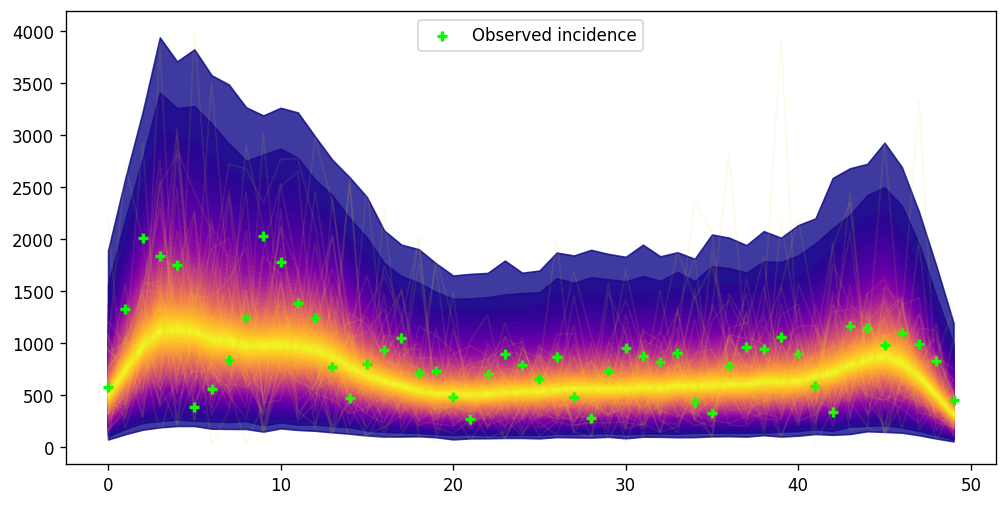
\includegraphics[width=11cm]{static/images/inc-model-ppc-plot-1-zero-mean.png}
  \caption{Posterior predictive of $\hat{c}$ for sample 1 with zero mean GP}
  \label{fig:incidence-posterior-1-zero-mean}
\end{figure}


\newpage
\section{The source code}

\subsection{Notebook initialization}

\input{generated/snippets/init-installs.tex}
\input{generated/snippets/init-imports.tex}

\subsection{Utilities}

\input{generated/snippets/config.tex}

\input{generated/snippets/utils-base-figure.tex}
\input{generated/snippets/utils-base-plotly.tex}
\input{generated/snippets/utils-base-matplotlib.tex}
\input{generated/snippets/utils-base-latex.tex}
\input{generated/snippets/utils-data-node.tex}
\input{generated/snippets/hyperparameters.tex}
% FIXME: resolve the unicode issues
% \input{generated/snippets/utils-cz-root.tex}
\input{generated/snippets/utils-adf-test}

\subsection{Data wrangling}

\input{generated/snippets/data-serial-interval-base.tex}
\input{generated/snippets/data-serial-interval-instances.tex}
\input{generated/snippets/data-serial-intervals-overview.tex}
\input{generated/snippets/data-serial-intervals-Omega.tex}
\input{generated/snippets/data-incidence.tex}
\input{generated/snippets/data-node-instances.tex}
\input{generated/snippets/data-largest-cities-plot.tex}
\input{generated/snippets/data-adf-test-prague.tex}
\input{generated/snippets/data-adf-test-brno-ostrava.tex}
\input{generated/snippets/data-seasonal-decomposition-figure.tex}
\input{generated/snippets/data-seasonal-decomposition-additive.tex}
\input{generated/snippets/data-seasonal-decomposition-multiplicative.tex}

\subsection{Incidence model}

\input{generated/snippets/incidence-log-transform-plot.tex}
\input{generated/snippets/theta-diff-plot.tex}
\input{generated/snippets/theta-diff-sample-windows-plot.tex}
\input{generated/snippets/theta-diff-histogram.tex}
\input{generated/snippets/theta-diff-qq-plot.tex}
\input{generated/snippets/theta-diff-ecdf-plot.tex}
% FIXME:
%\input{generated/snippets/theta-diff-ks-test.tex}
\input{generated/snippets/theta-diff-lilliefors-test.tex}
\input{generated/snippets/theta-diff-shapiro-wilk-test.tex}

\input{generated/snippets/inc-model-sample-incidence-figure.tex}
\input{generated/snippets/inc-model-sample-incidence-1.tex}
\input{generated/snippets/inc-model-sample-incidence-2.tex}
\input{generated/snippets/inc-model-sample-incidence-3.tex}

\input{generated/snippets/inc-model-build-func.tex}
\input{generated/snippets/inc-model-build-on-samples.tex}
\input{generated/snippets/inc-model-graphviz.tex}
\input{generated/snippets/inc-model-sampling-func.tex}
\input{generated/snippets/inc-model-sampling-1.tex}
\input{generated/snippets/inc-model-sampling-2.tex}
\input{generated/snippets/inc-model-sampling-3.tex}
\input{generated/snippets/inc-model-trace-figure.tex}
\input{generated/snippets/inc-model-sampling-trace-plot-1.tex}
\input{generated/snippets/inc-model-sampling-trace-plot-2.tex}
\input{generated/snippets/inc-model-sampling-trace-plot-3.tex}
\input{generated/snippets/inc-model-theta-posterior-figure.tex}
\input{generated/snippets/inc-model-theta-posterior-1.tex}
\input{generated/snippets/inc-model-theta-posterior-2.tex}
\input{generated/snippets/inc-model-theta-posterior-3.tex}

\input{generated/snippets/inc-model-pp-func.tex}
\input{generated/snippets/inc-model-ppc-1.tex}
\input{generated/snippets/inc-model-ppc-2.tex}
\input{generated/snippets/inc-model-ppc-3.tex}
\input{generated/snippets/inc-model-ppc-figure.tex}
\input{generated/snippets/inc-model-ppc-plot-1.tex}
\input{generated/snippets/inc-model-ppc-plot-2.tex}
\input{generated/snippets/inc-model-ppc-plot-3.tex}

\subsection{Risk model}

\input{generated/snippets/risk-model-fake-rt.tex}
\input{generated/snippets/risk-model-fake-sir.tex}
\input{generated/snippets/risk-model-fake-sir-plot.tex}
\input{generated/snippets/risk-model-fake-incidence.tex}
\input{generated/snippets/risk-model-fake-inference.tex}
\input{generated/snippets/risk-model-fake-inc-posterior.tex}
\input{generated/snippets/risk-model-prevalence-matrix.tex}
\input{generated/snippets/risk-model-helper-quantile-traces.tex}
\input{generated/snippets/risk-model-prevalence-plot.tex}
\input{generated/snippets/risk-model-reproduction-matrix.tex}
\input{generated/snippets/risk-model-reproduction-figure.tex}
\input{generated/snippets/risk-model-risk-est-plot.tex}


\subsection{The real data based example}

\input{generated/snippets/examples-incidence-estimate-func.tex}
\input{generated/snippets/examples-southbohemian-region-inference.tex}
\input{generated/snippets/examples-southbohemian-region-table.tex}
\input{generated/snippets/examples-southbohemian-region-crude.tex}


\end{document}
